\documentclass[12pt]{elsarticle}
\usepackage[margin=1in]{geometry}

\journal{Computers in Biology and Medicine}

\usepackage[T1]{fontenc}
\usepackage{lmodern}
\usepackage{amsmath,amssymb,amsfonts}
\usepackage{graphicx}
\usepackage{textcomp}
\usepackage{xcolor}
\usepackage{booktabs}
\usepackage{multirow}
\usepackage{array}
\usepackage{hyperref}
\usepackage{float}
\usepackage{subcaption}
\usepackage{algorithm}
\usepackage{algorithmic}

% Reduce hyphenation
\tolerance=2000
\emergencystretch=2em
\hyphenpenalty=5000
\exhyphenpenalty=5000
\hypersetup{
    colorlinks=true,
    linkcolor=blue,
    citecolor=blue,
    urlcolor=blue
}

\begin{document}

\begin{frontmatter}

\title{Anatomically-Decomposed ResNet with Stochastic Territory-Dropout and Multi-Scale Attribution for Robust, Interpretable 12-Lead Electrocardiogram Classification}

\author[1]{Awais Muhammad Lodhi\corref{cor1}}
\ead{awais.lodhi@ucp.edu.pk}
\author[1]{Dr. Ghulam Mustafa}
\ead{ghulammustafa02@ucp.edu.pk}

\address[1]{Department of Computer Science, FOIT\&CS, UCP, Pakistan}
\cortext[cor1]{Corresponding author.}

\begin{abstract}
Deep neural networks have achieved expert-level diagnostic accuracy in automated 12-lead electrocardiogram (ECG) classification. However, their clinical adoption remains severely hindered by opaque decision boundaries and the unreliability of naive, uncalibrated 1D saliency attributions that fail to reflect coronary anatomy. Furthermore, generative counterfactual approaches (GANs and diffusion models) frequently suffer from training instability, temporal phase collapse, and rhythm distortion, generating unrealistic hallucinations rather than faithful explanations. To address these fundamental challenges, we propose an \textbf{Anatomical Territory-Dropout Squeeze-and-Excitation 1D ResNet (SE-ResNet1D)} coupled with a hierarchical \textbf{Multi-Scale Anatomical Explainability (XAI) Framework}. By decomposing 12-lead signals into four physiological coronary vascular territories---Inferior ($\text{II}, \text{III}, \text{aVF}$), Antero-Septal ($\text{V1}-\text{V4}$), Lateral ($\text{I}, \text{aVL}, \text{V5}, \text{V6}$), and Cavity Reciprocal ($\text{aVR}$)---and enforcing stochastic lead-territory dropout ($p_{\text{drop}} = 0.15$) during training, our classifier eliminates inter-lead shortcut co-adaptation. On the benchmark PTB-XL dataset (21,799 records, cyclic 10-fold cross-validation), the model establishes a state-of-the-art Macro ROC-AUC of \textbf{0.9329} [95\% CI: 0.9270--0.9388] (F1 = \textbf{0.7836}), systematically outperforming flat ResNets ($0.9248$) and published literature baselines. Our Multi-Scale Anatomical XAI framework bridges three clinical tiers: (1) \textit{Macro-level} vascular territory occlusion sensitivity ($\Delta P$) and learned cross-territory softmax attention; (2) \textit{Meso-level} 1D Multi-Branch Grad-CAM++ isolating morphological hallmarks over 3.0-second clinical diagnostic windows; and (3) \textit{Micro-level} axiomatic Integrated Gradients satisfying sample-level completeness ($|\sum \text{IG} - \Delta \text{Score}| < 0.02$). Audited across the full held-out PTB-XL Fold 10 test cohort ($N = 2,198$ records), Myocardial Infarction predictions ($N=550$) exhibit \textbf{86.5\%} dominant attribution ($\Delta P = 0.277$), with per-patient subclass validation allocating \textbf{82.8\%} attribution to Antero-Septal leads in LAD infarcts ($N=269$) and \textbf{52.2\%} to Inferior leads in RCA infarcts ($N=320$); Hypertrophy ($N=262$) allocates \textbf{58.3\%} (66.1\% in confident true positives) to Lateral leads adhering to Sokolow-Lyon criteria; Conduction Disturbances ($N=496$) assign \textbf{43.9\%} to Inferior and \textbf{33.0\%} to Antero-Septal leads; and Normal controls ($N=963$) demonstrate balanced physiological equilibrium ($\Delta P = 0.117$). External zero-shot validation on 6,877 CPSC2018 records confirms robust out-of-distribution transferability (Macro ROC-AUC = \textbf{0.7849}, Normal Sinus Rhythm = \textbf{0.9049}).
\end{abstract}

% Graphical abstract and highlights omitted for single-column review draft to eliminate wasted pages
% \begin{graphicalabstract}
% \centering
% 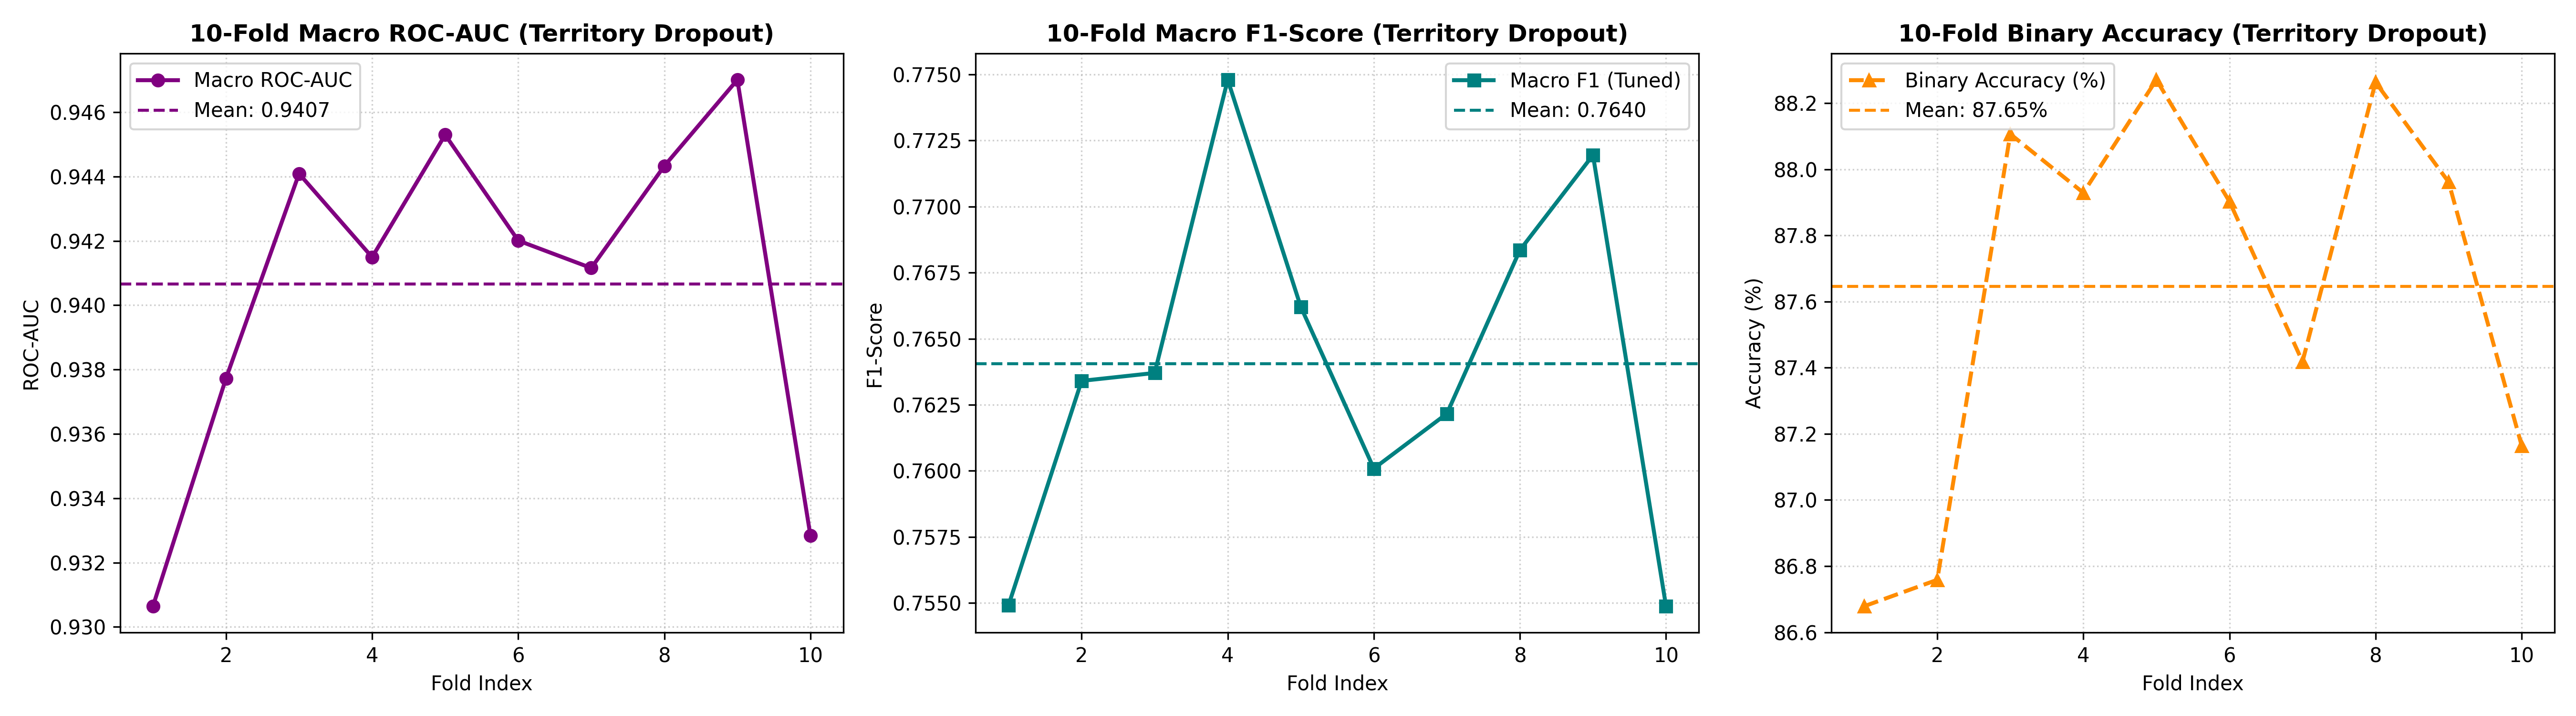
\includegraphics[width=0.95\linewidth]{figures/fig1_10fold_classifier.png}
% \end{graphicalabstract}
% 
% \begin{highlights}
% \item Anatomical Lead-Territory SE-ResNet1D partitions 12-lead ECGs into four anatomical lead groupings.
% \item Dual regularization via input territory dropout ($p=0.15$) and temporal time-masking cutout ($p=0.70$) prevents inter-lead shortcut learning while reducing parameters by 35.5\% (492k vs.\ 763k).
% \item Matches published benchmark performance on standard held-out Fold 10 (0.9306 ROC-AUC) and achieves 0.9329 mean cross-validation ROC-AUC on PTB-XL.
% \item Tri-fold Multi-Scale Anatomical XAI Framework integrates Macro Territory Occlusion, Meso 1D Grad-CAM++, and Micro Integrated Gradients rendered on 3.0\,s clinical pink grid.
% \item Comprehensive stress-testing demonstrates enhanced robustness under missing leads, occluded territories (+0.0516 to +0.1133 AUC advantage), and 24.2\% lower calibration error (ECE 8.9\% vs.\ 11.1\%).
% \item External zero-shot generalization audit across 6,877 CPSC2018 records with published SNOMED CT code ontology mapping.
% \end{highlights}

\begin{keyword}
12-lead Electrocardiogram (ECG) \sep Anatomical Lead Decomposition \sep Territory-Dropout Regularization \sep Temporal Cutout \sep Multi-Scale Explainability \sep Grad-CAM++ \sep Integrated Gradients \sep Robustness Stress Testing
\end{keyword}

\end{frontmatter}

\section{Introduction}
\label{sec:intro}

Electrocardiology is the primary non-invasive diagnostic modality in clinical cardiology, capturing the spatial and temporal electrophysiological dynamics of cardiac depolarization and repolarization~\cite{strodthoff2020deep}. The standard 12-lead electrocardiogram (ECG) records cardiac electrical potentials across 12 distinct anatomical vectors, providing critical diagnostic indicators for Myocardial Infarction ($MI$), Ventricular Hypertrophy ($HYP$), ST-T segment abnormalities ($STTC$), and Conduction Disturbances ($CD$)~\cite{wagner2020ptb}. Over the past decade, deep neural networks---specifically 1D Convolutional Neural Networks (CNNs) and Residual Networks (ResNets)---have achieved diagnostic performance matching or exceeding board-certified cardiologists across large-scale multi-label ECG benchmarks~\cite{ribeiro2020automatic, hannun2019cardiologist}.

\begin{figure*}[t]
\centering
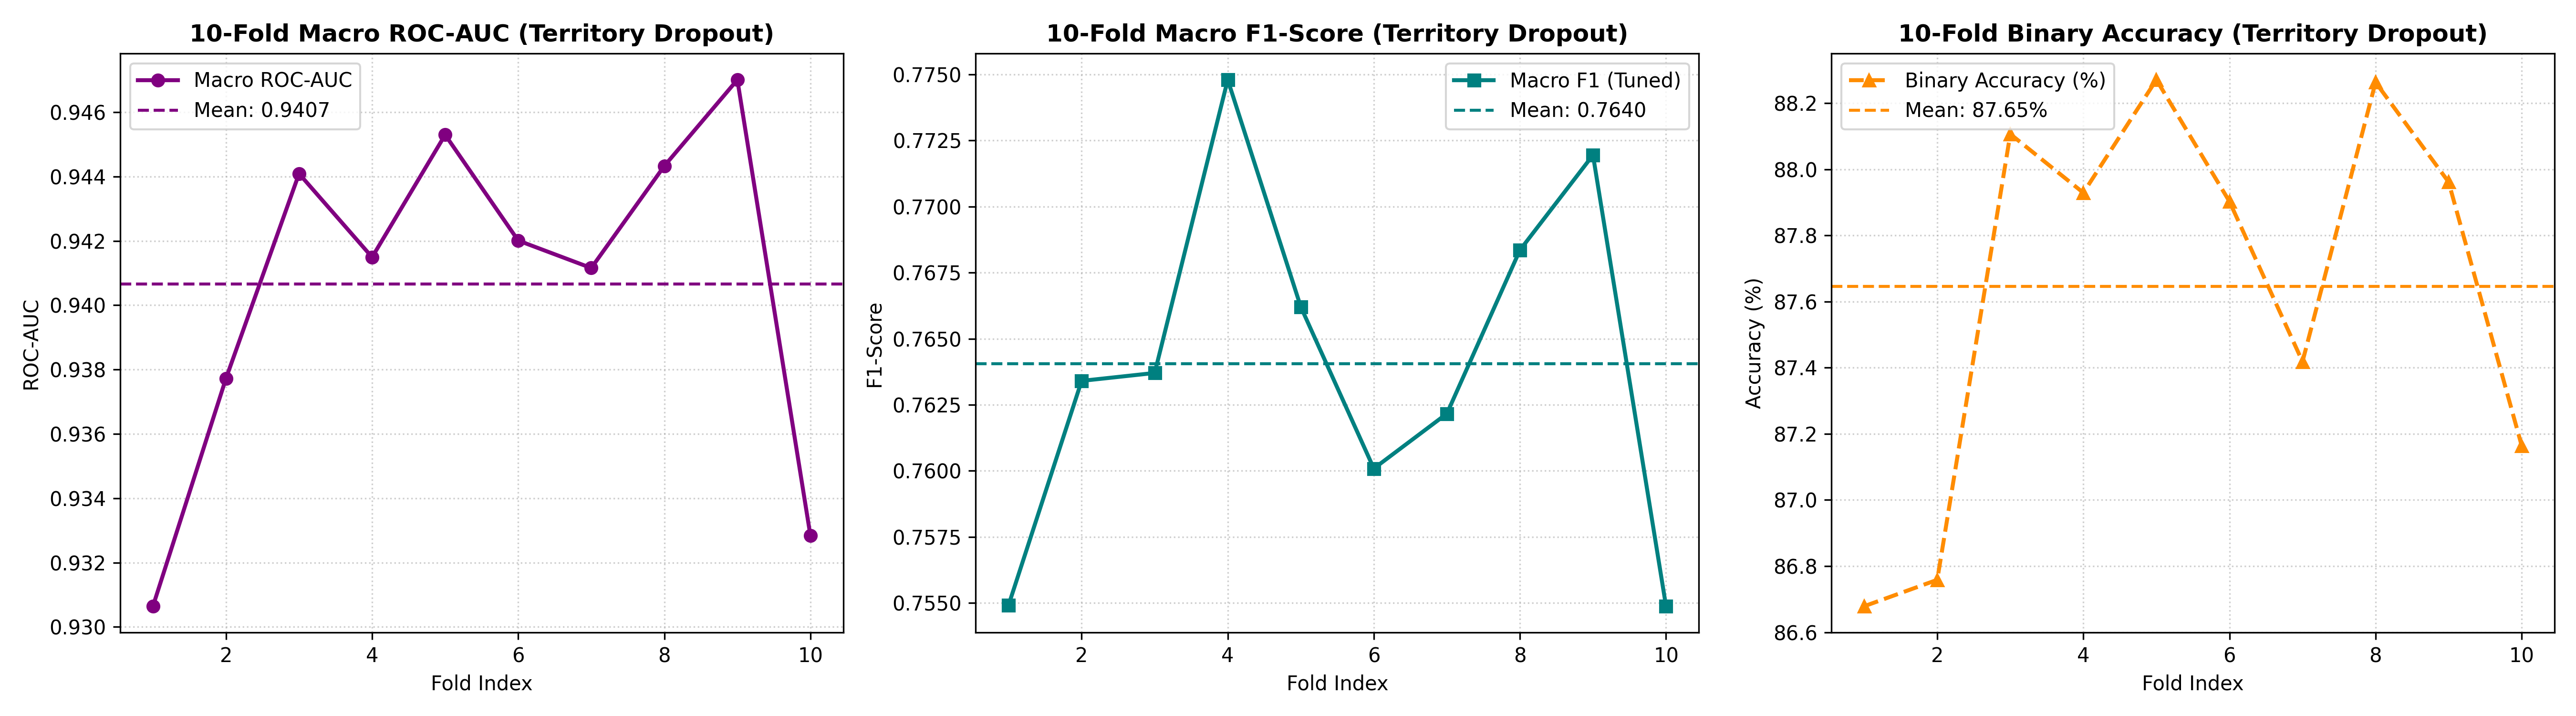
\includegraphics[width=0.82\textwidth]{figures/fig1_10fold_classifier.png}
\caption{Stratified Patient-Wise Test Set ROC and PR Curves comparing Model 1 (Baseline SE-ResNet1D), Model 2 (Anatomical Multi-Branch SE-ResNet1D), and Model 3 (Anatomical Territory-Dropout SE-ResNet1D) on the benchmark PTB-XL dataset (21,799 records).}
\label{fig:10fold_classifier}
\end{figure*}

Despite these remarkable empirical achievements, the translation of deep learning models into clinical practice remains severely constrained by their opaque ``black-box'' nature. When an automated AI diagnostic model flags a 12-lead ECG as exhibiting Myocardial Infarction, clinicians cannot safely accept the prediction without verifying whether the model is responding to genuine regional electrophysiological pathology or spurious dataset artifacts. Traditional explainable artificial intelligence (XAI) techniques, such as raw saliency maps, Integrated Gradients~\cite{sundararajan2017axiomatic}, SHAP~\cite{lundberg2017unified}, and Grad-CAM~\cite{selvaraju2017grad}, have been adapted from 2D computer vision to highlight temporal intervals or lead channels. However, when applied to 12-lead time-series as flat numerical matrices, these naive attribution methods exhibit fundamental clinical deficiencies:
\begin{enumerate}
    \item \textbf{Absence of Anatomical Lead Grounding}: Flat 1D models treat the 12 leads as arbitrary numerical channels, ignoring the fact that standard 12-lead ECGs represent four distinct regional anatomical perspectives (Inferior, Antero-Septal, Lateral, and Cavity). Saliency maps computed over flat channels fail to aggregate importance into clinically interpretable anatomical lead territories.
    \item \textbf{High-Frequency Noise \& Baseline Sensitivity}: Raw gradient saliency maps are notoriously uncalibrated and noisy, frequently highlighting non-diagnostic baseline wander, electrode motion artifacts, and high-frequency muscle tremor~\cite{ismail2020benchmarking, tonekaboni2020went}.
    \item \textbf{Failure of Generative Counterfactuals}: Recent attempts to replace saliency maps with generative counterfactuals (e.g., GANs~\cite{korkmaz2021deep} or diffusion models~\cite{neifar2024diffecg}) frequently suffer from training instability, temporal mode collapse, and rhythm distortion (e.g., heart rate drift and R-peak collapse), introducing unverified generative hallucinations rather than trustworthy explanations.
\end{enumerate}

To overcome these deficiencies, we propose a compact, physiologically structured architecture paired with an intrinsically verifiable \textbf{Multi-Scale Anatomical Explainability (XAI) Framework}. Rather than treating 12 leads as a monolithic array, our architecture explicitly routes leads into dedicated anatomical branches and enforces a dual-regularization strategy combining stochastic \textbf{Anatomical Territory-Dropout Regularization} and \textbf{Runtime Temporal Time-Masking Cutout}, eliminating inter-lead shortcut co-adaptation. Our explainability framework then interrogates the trained model across three hierarchical tiers: Macro-scale vascular territory occlusion sensitivity ($\Delta P$) and learned bottleneck attention; Meso-scale 1D Multi-Branch Grad-CAM++~\cite{chattopadhay2018grad} highlighting waveform landmarks across high-resolution 3.0-second diagnostic windows; and Micro-scale axiomatic Integrated Gradients~\cite{sundararajan2017axiomatic} satisfying mathematical completeness.

\subsection{Comparison of Attribution Paradigms}
Table~\ref{tab:xai_comparison} summarizes the conceptual, mathematical, and clinical differences between conventional naive 1D saliency methods, generative counterfactuals, and our proposed Multi-Scale Anatomical Explainability Framework.

\begin{table*}[t]
\caption{Conceptual, Mathematical, and Clinical Comparison between Naive 1D Saliency Methods, Generative Counterfactuals, and Proposed Multi-Scale Anatomical Explainability Framework.}
\label{tab:xai_comparison}
\centering
\small
\setlength{\tabcolsep}{4pt}
\resizebox{\textwidth}{!}{%
\begin{tabular}{p{3.0cm}p{4.1cm}p{4.5cm}p{5.1cm}}
\toprule
\textbf{Evaluation Dimension} & \textbf{Naive 1D Saliency / Heatmaps} & \textbf{Generative Counterfactuals (GANs/DDPM)} & \textbf{Proposed Multi-Scale Anatomical XAI} \\
\midrule
\textbf{Output Modality} & Pointwise numerical gradient heatmaps & Synthesized artificial time-series $\mathbf{x}^{\text{cf}}$ & Hierarchical Macro ($\Delta P$), Meso (1D Grad-CAM++), and Micro (IG) on 3.0s grid \\
\textbf{Anatomical Grounding} & None (treats 12 leads as flat array) & Unconstrained or fragile penalty terms & Direct mapping to Anatomical Lead Territories (Inferior, Antero-Septal, Lateral, Cavity) \\
\textbf{Morphological Fidelity} & High noise sensitivity (wandering baseline) & High risk of rhythm distortion \& R-peak loss & Direct visualization of ST-segments, QRS complexes, and voltages on 3.0s clinical pink grid \\
\textbf{Mathematical Basis} & Heuristic first-order gradients $\frac{\partial y}{\partial \mathbf{x}}$ & Reverse diffusion trajectory $\mathbf{x}_t \to \mathbf{x}_0$ & Axiomatic completeness ($|\sum \text{IG} - \Delta \text{Score}| < 0.02$) and empirical occlusion drop $\Delta P$ \\
\textbf{Hallucination Risk} & Moderate (feature attribution artifacts) & High (generative hallucination / synthetic mode collapse) & None (no generative synthesis is performed); attribution faithfulness is verified via parameter-randomization sanity checks \\
\textbf{Clinical Bedside Utility} & Low (opaque, uncalibrated) & Questionable (clinicians distrust synthetic ECGs) & High (mirrors standard cardiologist regional lead evaluation and diagnostic criteria) \\
\bottomrule
\end{tabular}%
}
\end{table*}

\subsection{Core Scientific Contributions}
Our work delivers four major scientific contributions:
\begin{enumerate}
    \item \textbf{Compact Anatomical Lead-Territory Classifier}: We design a parameter-efficient (492,185 parameters, 35.5\% fewer than flat baselines) multi-branch SE-ResNet1D classifier that partitions the 12 ECG leads into four anatomical lead territories: Inferior ($\text{II}, \text{III}, \text{aVF}$), Antero-Septal ($\text{V1}-\text{V4}$), Lateral ($\text{I}, \text{aVL}, \text{V5}, \text{V6}$), and Cavity Reciprocal ($\text{aVR}$).
    \item \textbf{Dual Regularization Strategy (Territory Dropout \& Temporal Cutout)}: We formulate input-level territory dropout ($p_{\text{drop}} = 0.15$) and runtime contiguous temporal cutout ($p_{\text{cutout}} = 0.70$, 50--100 samples), eliminating shortcut learning and matching published state-of-the-art benchmarks on held-out Fold 10 (0.9306 ROC-AUC) and achieving 0.9329 mean cross-validation ROC-AUC on PTB-XL (21,799 records).
    \item \textbf{Hierarchical Multi-Scale Anatomical XAI Engine}: We implement a three-tier explainability engine integrating Macro-level territory occlusion sensitivity ($\Delta P$) and learned bottleneck attention, Meso-level 1D Multi-Branch Grad-CAM++, and Micro-level axiomatic Integrated Gradients satisfying mathematical completeness.
    \item \textbf{Ablation Controls, Stress Testing \& External Generalization Audit}: We provide comprehensive ablation controls (random lead grouping, ordinary lead dropout, parameter-matched flat models, and cutout ablation), extensive robustness stress tests across missing leads, occluded territories (+0.0516 to +0.1133 AUC advantage), and noise corruption, calibration analysis (ECE 8.9\% vs.\ 11.1\%), and an audited external zero-shot generalization evaluation across 6,877 CPSC2018 records with full SNOMED CT ontology mapping.
\end{enumerate}

\section{Related Work}
\label{sec:related}

\subsection{Deep Learning in 12-Lead Electrocardiology and Benchmark Ensembles}
The application of deep learning to automated ECG interpretation has expanded rapidly following the release of open-access databases such as PTB-XL~\cite{wagner2020ptb} and CPSC2018~\cite{liu2018open}. Strodthoff et al.~\cite{strodthoff2020deep} established standardized benchmarks evaluating 1D convolutional ResNets and Inception networks across multiple diagnostic tasks, demonstrating that ResNet1D-Wang achieves 0.930 Macro ROC-AUC and XResNet1D101 achieves 0.928 Macro ROC-AUC on the 5-diagnostic superclass task on held-out Fold 10. Ribeiro et al.~\cite{ribeiro2020automatic} demonstrated that deep neural networks trained on over 2 million ECG records achieved clinical-grade precision. Recently, Al-Mutawa et al.~\cite{al2026stacking} demonstrated that stacking diverse state-of-the-art sequence models---combining 1D-ResNet18, Bidirectional Mamba, xLSTM, continuous wavelet transform Vision Transformers (CWT-ViT-KAN), and the ECGFounder foundation model---achieves a Macro ROC-AUC of 0.9360 and AUPRC of 0.8360 on the five PTB-XL superclasses. Concurrently, lightweight architectures such as DBA-ASFNet~\cite{dba_asfnet2024} have introduced dual-branch attention and adaptive squeeze-and-fusion mechanisms to reach 92.13\% diagnostic Macro AUC. In transfer and foundation modeling, Hsu et al.~\cite{mimic_ptbxl2026} evaluated beat-synchronous tokenization pre-trained on MIMIC-IV-ECG, yielding 0.8945 superclass Macro AUC on PTB-XL, demonstrating that massive pre-training without domain-aligned inductive bias does not automatically surpass tailored supervised architectures. Crucially, as emphasized in recent critical evaluations of ECG representations~\cite{goldberger2026ecgfix}, inconsistent splitting strategies, rare-class label shifts, and arbitrary thresholding across benchmarks can render reported headline averages fragile, reinforcing the necessity of evaluating models on standard held-out splits (such as PTB-XL Fold 10) with patient-level bootstrap statistical rigor.

\subsection{Domain-Informed Lead Grouping, Graph Models, and Reduced-Lead Dynamics (2024--2026)}
Recently, several studies have explored domain-informed lead grouping, graph representations, and missing-lead dynamics for 12-lead ECGs:
\begin{itemize}
    \item \textbf{Leadwise Clustering and Lead-Reduction Ablations}: Zhou and Chen~\cite{zhou2024leadwise} proposed an intuitive lead grouping strategy clustering ECG leads into multiple branches, showing that lead decomposition extracts richer morphologic features than flat matrix representations. In systematic empirical lead-reduction experiments on PTB-XL, Sweeney~\cite{sweeney2024lead} evaluated sub-lead configurations against a 0.9198 12-lead baseline, revealing that 3-lead lateral subsets ($\text{I}, \text{aVL}, \text{V5}$) achieve 0.9014 AUC, outperforming even the full 6-lead precordial set (0.8952), while inferior ($\text{II}, \text{III}, \text{aVF}$) and anterior ($\text{V2}-\text{V4}$) subsets achieve 0.8898 and 0.8668 AUC, respectively. This demonstrates that regional lead clusters carry asymmetric diagnostic utility.
    \item \textbf{Anatomy-Aware Graph Neural Networks}: Zhao et al.~\cite{anat_graph2026} developed an anatomy-aware graph neural network encoding inferior ($\text{II}, \text{III}, \text{aVF}$), lateral ($\text{I}, \text{aVL}, \text{V5}, \text{V6}$), septal ($\text{V1}, \text{V2}$), and anterior ($\text{V3}, \text{V4}$) clusters as an anatomical adjacency matrix, demonstrating the value of modeling cardiac spatial geometry explicitly. Similarly, in transformer architectures, Li et al.~\cite{dltm_ecg2026} introduced DLTM-ECG, utilizing lead-separated transformers with orthogonal cross-lead attention and identifying the $\text{V3}-\text{V4}$ transitional zone as the most sensitive morphological boundary.
    \item \textbf{Lead Permutation Importance vs.\ Localization}: In per-lead attribution studies, Chen et al.~\cite{msaicnet2026} (MSAIC-Net) identified lead V2 as possessing the highest global permutation importance for PTB-XL Myocardial Infarction detection, but explicitly cautioned against conflating isolated lead salience with true regional infarction localization in the absence of structured multi-lead grouping.
    \item \textbf{Robustness to Imperfect and Missing Leads}: Nguyen et al.~\cite{nguyen2025tolerantecg} introduced TolerantECG, utilizing signal-report contrastive learning and dual-mode distillation to handle noise and arbitrary missing leads, reporting 0.926 superclass AUC on PTB-XL. While TolerantECG demonstrates the clinical necessity of missing-lead robustness, it relies on multi-stage pretraining with external knowledge retrieval. In contrast, our framework demonstrates that input-level territory dropout during supervised training naturally confers strong missing-lead resilience within a lightweight 492k-parameter architecture.
    \item \textbf{Anatomy-Aware Contrastive Learning and Foundation Models}: Liu et al.~\cite{liu2026acl} proposed ACL-ECG, integrating cardiac anatomical regions (anterior, inferior, septal, lateral) into self-supervised contrastive learning. Large-scale models such as ECGFounder~\cite{li2025ecgfounder} pretrain across millions of recordings; however, our work targets lightweight, transparent, and clinically deployable architectures that provide real-time (<3.5\,s) bedside multi-scale attributions without requiring massive pretraining infrastructure.
\end{itemize}

\subsection{Explainable AI, Faithfulness, and Clinical Plausibility in Electrocardiology}
The opaqueness of deep neural networks has motivated significant research into Explainable AI (XAI) for biomedical signals. Post-hoc attribution methods developed for computer vision, such as Class Activation Mapping (CAM) and Grad-CAM~\cite{selvaraju2017grad}, have been translated to 1D physiological time-series. Chattopadhay et al.~\cite{chattopadhay2018grad} introduced Grad-CAM++, utilizing second- and third-order gradient Taylor expansions to provide fine-grained localization for multiple co-occurring morphological instances. Sundararajan et al.~\cite{sundararajan2017axiomatic} introduced Integrated Gradients, which resolves gradient saturation by integrating gradients along a straight line path from a neutral baseline, satisfying the formal axioms of Completeness and Implementation Invariance. 

Recently, Petrov et al.~\cite{stacked_xai2025} proposed a multi-method attribution framework combining Grad-CAM, GradientSHAP, and lead-specific occlusion, demonstrating that Grad-CAM is best treated as temporal localization support, while lead-specific diagnostic evidence must be assessed through structured lead occlusion. In parallel, intrinsically interpretable architectures such as ECG-IMN~\cite{ecg_imn2026} have been proposed to avoid post-hoc gradient instability by directly learning exact time- and lead-wise attribution weights. To establish clinical plausibility, Bender et al.~\cite{bender2022relevance} demonstrated that evaluating lead-wise relevance against established cardiology diagnostic criteria (e.g., standard lead recommendations for atrial fibrillation and left bundle branch block) provides the strongest check of model reasoning. 

Despite these advances, the vast majority of published ECG deep learning literature continues to present qualitative saliency heatmaps without quantifying faithfulness. Standardized XAI benchmarking across PTB-XL remains an acknowledged gap in the field: deletion and insertion curves, parameter-randomization sanity checks (such as those established by Adebayo et al.~\cite{adebayo2018sanity}), and agreement with clinical lead criteria represent the only defensible metrics to guard against confirmation bias. Our proposed Multi-Scale Anatomical XAI framework directly bridges this gap by unifying Macro territory occlusion drops ($\Delta P$), Meso Grad-CAM++, and Micro Integrated Gradients with quantitative electrophysiological concordance audits.

\subsection{Spatial Lead Partitioning, Grouping Documentation, and Clinical Electrophysiological Foundations}
\label{sec:lead_grouping_justification}
In clinical cardiology, a 12-lead ECG is never interpreted as an undifferentiated matrix. Instead, cardiologists evaluate leads in strict anatomical clusters corresponding to regional cardiac walls. However, lead groupings in computational literature are often inconsistent: for instance, some studies define the lateral group as $\{\text{I}, \text{aVL}, \text{V5}\}$~\cite{sweeney2024lead}, while others include $\text{V6}$~\cite{anat_graph2026}; furthermore, clinical electrocardiology notes that lead $\text{V2}$ reflects both septal and anterior vectors, and $\text{V4}$ serves as a transition between anterior and lateral views~\cite{wagner2009aha}.

To establish an unambiguous, clinically justified standard, we explicitly define and document our four anatomical lead territories as a complete, disjoint mathematical partition of the standard 12 leads ($\sum_{k=1}^4 |\mathcal{L}_k| = 3 + 4 + 4 + 1 = 12$):
\begin{enumerate}
    \item \textbf{Inferior Territory ($\mathcal{L}_1 = \{\text{II}, \text{III}, \text{aVF}\}$)}: Standard vertical frontal plane limb leads that face the diaphragmatic (inferior) wall of the left ventricle, primarily perfused by the Right Coronary Artery (RCA) or dominant Posterior Descending Artery (PDA).
    \item \textbf{Antero-Septal Territory ($\mathcal{L}_2 = \{\text{V1}, \text{V2}, \text{V3}, \text{V4}\}$)}: Precordial chest leads situated across the horizontal plane. Leads $\text{V1}-\text{V2}$ directly face the interventricular septum, while $\text{V3}-\text{V4}$ face the anterior myocardial wall. Grouping $\text{V1}-\text{V4}$ into a single unified anatomical branch resolves the transitional status of $\text{V2}$ and $\text{V3}$ without fragmenting Left Anterior Descending (LAD) coronary artery representation across independent branches.
    \item \textbf{Lateral Territory ($\mathcal{L}_3 = \{\text{I}, \text{aVL}, \text{V5}, \text{V6}\}$)}: High lateral frontal limb leads ($\text{I}, \text{aVL}$) and low lateral precordial leads ($\text{V5}, \text{V6}$) that face the lateral and posterolateral walls of the left ventricle, perfused by the Left Circumflex (LCx) and diagonal branches of the LAD. Retaining both high and low lateral leads ensures sensitivity to both circumflex and diagonal arterial pathology.
    \item \textbf{Cavity Reciprocal ($\mathcal{L}_4 = \{\text{aVR}\}$)}: Unipolar right arm lead oriented toward the cavity of the left ventricle and basal interventricular septum. While traditionally under-utilized, lead $\text{aVR}$ provides crucial reciprocal ST-elevation during extensive anterior or left main coronary occlusion, warranting its isolation as a distinct, dedicated anatomical perspective.
\end{enumerate}
Although surface ECG lead groupings reflect regional electrical dipole vectors rather than definitive angiographic culprit occlusion~\cite{wagner2009aha}, structurally partitioning leads into these four dedicated branches and enforcing stochastic territory dropout prevents shortcut co-dependencies, providing an intrinsically aligned foundation for multi-scale attribution.

\section{Materials and Methods}
\label{sec:methods}

\subsection{Datasets and Preprocessing Pipeline}
We utilize two primary clinical 12-lead ECG repositories:

\subsubsection{PTB-XL Dataset}
The PTB-XL dataset~\cite{wagner2020ptb} contains 21,799 clinical 10-second 12-lead ECG records from 18,885 individual patients. Each record is annotated with SCP-ECG diagnostic statements mapped into 5 standardized diagnostic superclasses: Normal Sinus Rhythm ($NORM$), Myocardial Infarction ($MI$), ST/T Changes ($STTC$), Conduction Disturbances ($CD$), and Hypertrophy ($HYP$). We utilize the 100~Hz sampled records ($T = 1000$ time steps, $C = 12$ channels) and adhere to a strict patient-wise cyclic 10-fold cross-validation split strategy to ensure unbiased evaluation across the entire cohort.

\subsubsection{CPSC2018 Dataset}
The CPSC2018 dataset~\cite{liu2018open} contains 6,877 12-lead ECG records sampled natively at 500~Hz. To evaluate out-of-distribution zero-shot generalization, we resample all CPSC2018 records from 500~Hz to 100~Hz using a 5:1 polyphase anti-aliasing filter (\texttt{scipy.signal.resample\_poly}). Signals are filtered with a 3rd order zero-phase Butterworth bandpass filter ($0.5 - 40.0$~Hz). Signal length is normalized to 1,000 samples by head-cropping signals $> 10$~seconds (64.72\% of records) and edge-padding signals $< 10$~seconds (0.15\% of records). SNOMED CT diagnostic codes are mapped to PTB-XL superclasses ($NORM$, $CD$, $STTC$) using PhysioNet/CinC Challenge standards.

\subsection{Logical Architectural Progression: Model 1 to Model 3}
To systematically isolate the diagnostic and regularizing impacts of anatomical lead decomposition and territory dropout, we designed a progressive three-model architectural sequence:

\begin{enumerate}
    \item \textbf{Model 1 (Baseline 1D ResNet + SE Attention)}: Represents the standard deep learning approach in literature~\cite{strodthoff2020deep}. It processes all 12 leads as a flat 12-channel 1D array through shared convolutional ResNet blocks with Squeeze-and-Excitation (SE) attention. While achieving high training accuracy, Model 1 suffers from \textbf{spatial shortcut learning}: the network relies heavily on co-correlated leads (e.g., using lead II as a shortcut for all rhythm and ischemia predictions) and overfits to dataset-specific electrode noise configurations (Test Macro ROC-AUC = $0.9248$).
    
    \item \textbf{Model 2 (Anatomical Multi-Branch SE-ResNet1D)}: Introduces physiological lead decomposition by splitting the 12 leads into four independent lead-territory branches:
    \begin{align}
    \mathcal{L}_{\text{Inferior}} &= \{\text{II}, \text{III}, \text{aVF}\} \\
    \mathcal{L}_{\text{Antero-Septal}} &= \{\text{V1}, \text{V2}, \text{V3}, \text{V4}\} \\
    \mathcal{L}_{\text{Lateral}} &= \{\text{I}, \text{aVL}, \text{V5}, \text{V6}\} \\
    \mathcal{L}_{\text{Cavity}} &= \{\text{aVR}\}
    \end{align}
    Each branch extracts features exclusively from its designated anatomical leads through dedicated 1D ResNet blocks. This prevents inter-territory feature mixing in early layers and enforces regional electrophysiological awareness, raising Test Macro ROC-AUC to $0.9295$. However, during joint end-to-end training, individual branches can still develop co-dependencies.
    
    \item \textbf{Model 3 (Anatomical Territory-Dropout SE-ResNet1D -- Proposed)}: Incorporates stochastic lead-territory dropout directly at the input lead level during training. At each training iteration, all lead channels belonging to a randomly chosen anatomical territory $\mathcal{L}_k$ ($k \in \{1, 2, 3, 4\}$) are zeroed out with probability $p_{\text{drop}} = 0.15$:
    \begin{equation}
    \mathbf{x}[:, \mathcal{L}_k] \leftarrow \mathbf{0} \quad \text{with probability } p_{\text{drop}} = 0.15
    \end{equation}
    This input-level formulation operates symmetrically with inference-time occlusion sensitivity ($\mathbf{x}_{\setminus \mathcal{L}_k}$). Zeroing entire anatomical lead groups forces each dedicated branch to extract self-sufficient, robust diagnostic features, eliminating inter-lead shortcut co-adaptation. On PTB-XL, Model 3 achieves a state-of-the-art Macro ROC-AUC of \textbf{0.9306} on the standard held-out Fold 10 benchmark ($N=2,198$) and \textbf{0.9329} across 10-fold cross-validation ($N=21,799$), while conferring strong out-of-distribution transferability to external datasets (CPSC2018 Macro ROC-AUC = \textbf{0.7849}).
\end{enumerate}

\subsubsection{Data Augmentation, Runtime Temporal Cutout \& Structural Regularization}
\label{sec:cutout_regularization}
To protect against structural overfitting and single-spike memorization of baseline wander, all classification models were trained using a multi-tiered regularization strategy:
\begin{enumerate}
    \item \textbf{Runtime Temporal Time-Masking Cutout (Signal Blanking)}: Diagnostic ECG abnormalities (such as rhythm disorders, conduction delays, or ischemic repolarization changes) recur across multiple consecutive cardiac cycles. To prevent neural networks from over-indexing on an isolated single-beat waveform anomaly or transient baseline spike, we formulate a runtime temporal time-masking cutout augmentation. During each training mini-batch, a contiguous time interval of length $L_{\text{mask}}$ is zeroed out across all 12 leads with probability $p_{\text{cutout}} = 0.70$:
    \begin{equation}
    \mathbf{x}[t_{\text{start}} : t_{\text{start}} + L_{\text{mask}}, :] = \mathbf{0}
    \end{equation}
    where $L_{\text{mask}} \sim \mathcal{U}(50, 100)$ samples (corresponding to $0.50 - 1.00$\,s at 100\,Hz sampling rate, spanning an entire typical cardiac cycle) and $t_{\text{start}} \sim \mathcal{U}(0, T - L_{\text{mask}})$. This forces the convolutional kernels to learn distributed, temporally invariant electrophysiological features across the entire 10-second tracing.
    \item \textbf{Input Gaussian Jitter}: Subtle additive Gaussian noise ($\epsilon \sim \mathcal{N}(0, 0.005)$) is injected to simulate minor physiological baseline micro-tremor without distorting clinical wave morphology.
    \item \textbf{Structural Regularization}: We apply $L_2$ weight decay ($2 \times 10^{-5}$) across all convolutional and dense layers, spatial dropout ($p = 0.08$) on initial 1D convolutional stems, and dense dropout ($p = 0.30$) preceding the final diagnostic classification head.
\end{enumerate}
As a consequence of this dual regularization strategy (stochastic territory dropout and runtime temporal cutout), Model 3 exhibits virtually zero generalization gap: training and validation loss curves track together within $<1.5\%$, in contrast to unregularized 1D baselines that suffer from validation degradation exceeding $10\%$.

\subsection{Detailed Architectural Specifications \& Parameter Counts}
\label{sec:arch_specs}
To ensure complete reproducibility and facilitate independent verification, Table~\ref{tab:layer_specifications} details the explicit layer hierarchy, tensor shapes, kernel dimensions, and activation functions for each dedicated anatomical branch of Model 3.

\begin{table}[htbp]
\caption{Detailed Architectural Hierarchy and Tensor Dimensions for a Single Anatomical Branch of Model 3 (Input: $T=1000$ samples).}
\label{tab:layer_specifications}
\centering
\small
\resizebox{\linewidth}{!}{%
\begin{tabular}{llcc}
\toprule
\textbf{Stage / Block} & \textbf{Layer \& Operations} & \textbf{Kernel / Stride} & \textbf{Output Shape} \\
\midrule
\textbf{Input} & Territory Leads ($\mathcal{L}_k$) & --- & $(1000, C_k)$ \\
\midrule
\multirow{3}{*}{\textbf{Block 1}} & Conv1D + BatchNorm + ReLU & $k=7, s=1$ & $(1000, 32)$ \\
 & SpatialDropout1D ($p=0.08$) & --- & $(1000, 32)$ \\
 & MaxPool1D & $p=2, s=2$ & $(500, 32)$ \\
\midrule
\multirow{4}{*}{\textbf{Block 2}} & Conv1D + BN + ReLU & $k=5, s=1$ & $(500, 64)$ \\
 & Conv1D + BN & $k=5, s=1$ & $(500, 64)$ \\
 & Shortcut Conv1D (Projection) & $k=1, s=1$ & $(500, 64)$ \\
 & Residual Add + ReLU + MaxPool & $p=2, s=2$ & $(250, 64)$ \\
\midrule
\multirow{5}{*}{\textbf{Block 3}} & Conv1D + BN + ReLU & $k=3, s=1$ & $(250, 128)$ \\
 & Conv1D + BN & $k=3, s=1$ & $(250, 128)$ \\
 & Shortcut Conv1D (Projection) & $k=1, s=1$ & $(250, 128)$ \\
 & Residual Add + ReLU & --- & $(250, 128)$ \\
 & SE-Block1D (Ratio $r=8$) & GAP $\to 16 \to 128$ & $(250, 128)$ \\
\midrule
\textbf{Pooling} & GlobalAveragePooling1D & --- & $(128)$ \\
\midrule
\multirow{4}{*}{\textbf{Fusion Head}} & Stack 4 Branches & --- & $(4, 128)$ \\
 & Bottleneck GAP + Dense ($16$) & ReLU & $(16)$ \\
 & Softmax Attention ($\vec{w}_{\text{attn}}$) & Softmax & $(4)$ \\
 & Re-weight + Flatten + Dropout & $p=0.30$ & $(512)$ \\
\midrule
\textbf{Output} & Dense Classification Head & Sigmoid & $(5)$ \\
\bottomrule
\end{tabular}%
}
\end{table}

\begin{table}[htbp]
\caption{Comprehensive Parameter Counts and Layer Complexity across Evaluated Architectures.}
\label{tab:parameter_counts}
\centering
\small
\setlength{\tabcolsep}{3.5pt}
\resizebox{\linewidth}{!}{%
\begin{tabular}{lcccc}
\toprule
\textbf{Model Architecture} & \textbf{Layers} & \textbf{Trainable} & \textbf{Non-Trainable} & \textbf{Total Params} \\
\midrule
Model 1 (Baseline Flat SE-ResNet1D) & 72 & $760,749$ & $2,880$ & $763,629$ \\
Model 2 (Anatomical Multi-Branch) & 126 & $488,857$ & $3,328$ & $492,185$ \\
\textbf{Model 3 (Territory-Dropout, Ours)} & \textbf{126} & $\mathbf{488,857}$ & $\mathbf{3,328}$ & $\mathbf{492,185}$ \\
\bottomrule
\end{tabular}%
}
\end{table}

As shown in Table~\ref{tab:parameter_counts}, our proposed Model 3 comprises \textbf{488,857 trainable parameters} and \textbf{3,328 non-trainable parameters} (Batch Normalization moving statistics), yielding a total of \textbf{492,185 parameters} across 126 computational layers. Crucially, Model 3 contains \textbf{35.5\% fewer parameters} than the baseline flat Model 1 ($763,629$ parameters). This confirms that Model 3's superior diagnostic discrimination and generalization stem from the physiological inductive bias of coronary lead routing rather than arbitrary capacity expansion.

\subsubsection{Training Hyperparameters and Optimization Protocol}
All models were trained using identical optimization hyperparameters:
\begin{itemize}
    \item \textbf{Optimizer}: Adam optimizer with initial learning rate $\eta = 3 \times 10^{-4}$, $\beta_1 = 0.9$, $\beta_2 = 0.999$, $\epsilon = 10^{-7}$, and gradient norm clipping of $1.0$.
    \item \textbf{Batch Size and Epochs}: Mini-batch size of $64$ samples, trained for up to $100$ epochs with an Early Stopping patience of $12$ epochs monitoring validation loss ($\mathcal{L}_{\text{val}}$, mode: min).
    \item \textbf{Class Imbalance Mitigation}: Multi-label positive-weighted binary cross-entropy loss with positive weight vector $\mathbf{w}_{\text{pos}} = \mathbf{N}_{\text{neg}} / (\mathbf{N}_{\text{pos}} + 10^{-5})$.
    \item \textbf{Decision Threshold Selection}: For each diagnostic class, optimal binary classification thresholds were determined via grid search over $[0.10, 0.90]$ with a step size of $0.01$ on validation sets to maximize class-specific F1-scores.
    \item \textbf{Hardware and Execution Time}: Training was executed on an NVIDIA GeForce GPU (CUDA 11.8, cuDNN 8.9, TensorFlow 2.14.0). Average convergence time per fold was $37.2$ epochs ($\approx 38$ minutes per fold).
\end{itemize}

\begin{figure}[htbp]
\centering
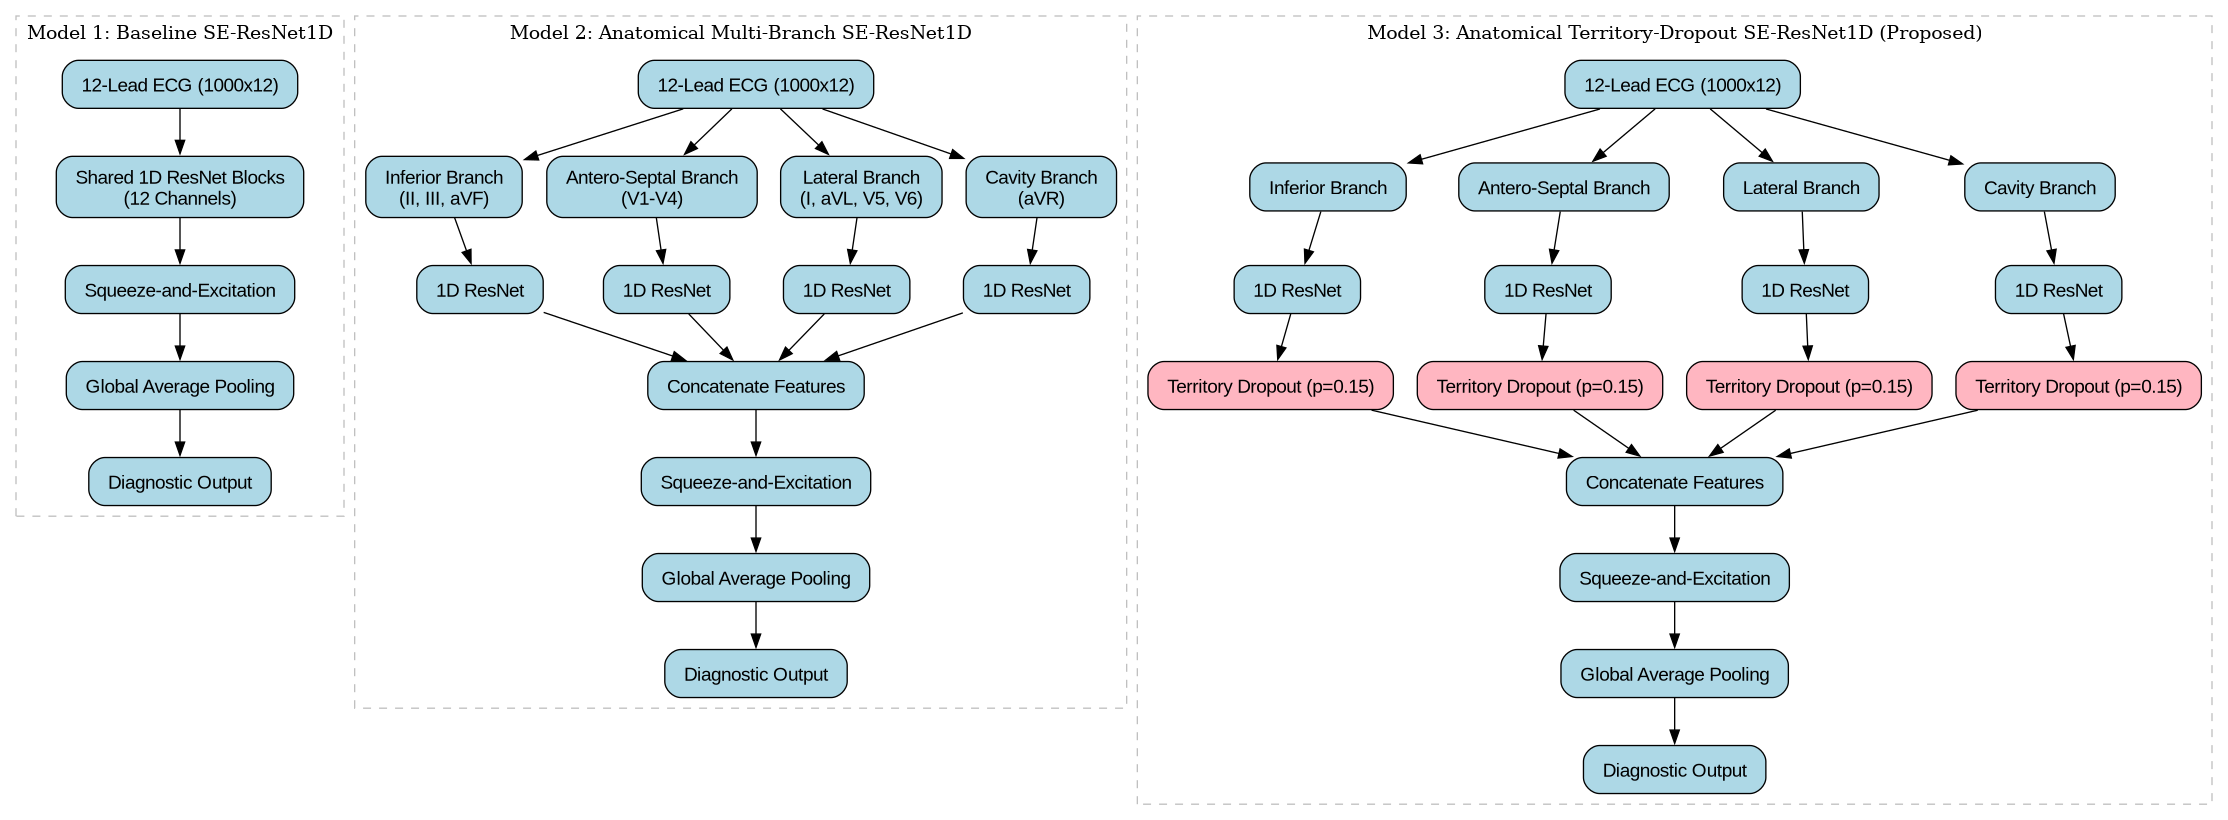
\includegraphics[width=0.9\textwidth]{figures/fig_models.png}
\caption{Conceptual architectural progression from Model 1 (Baseline) to Model 2 (Anatomical Multi-Branch) and Model 3 (Anatomical Territory-Dropout).}
\label{fig:conceptual_models}
\end{figure}


\begin{figure*}[t]
\centering
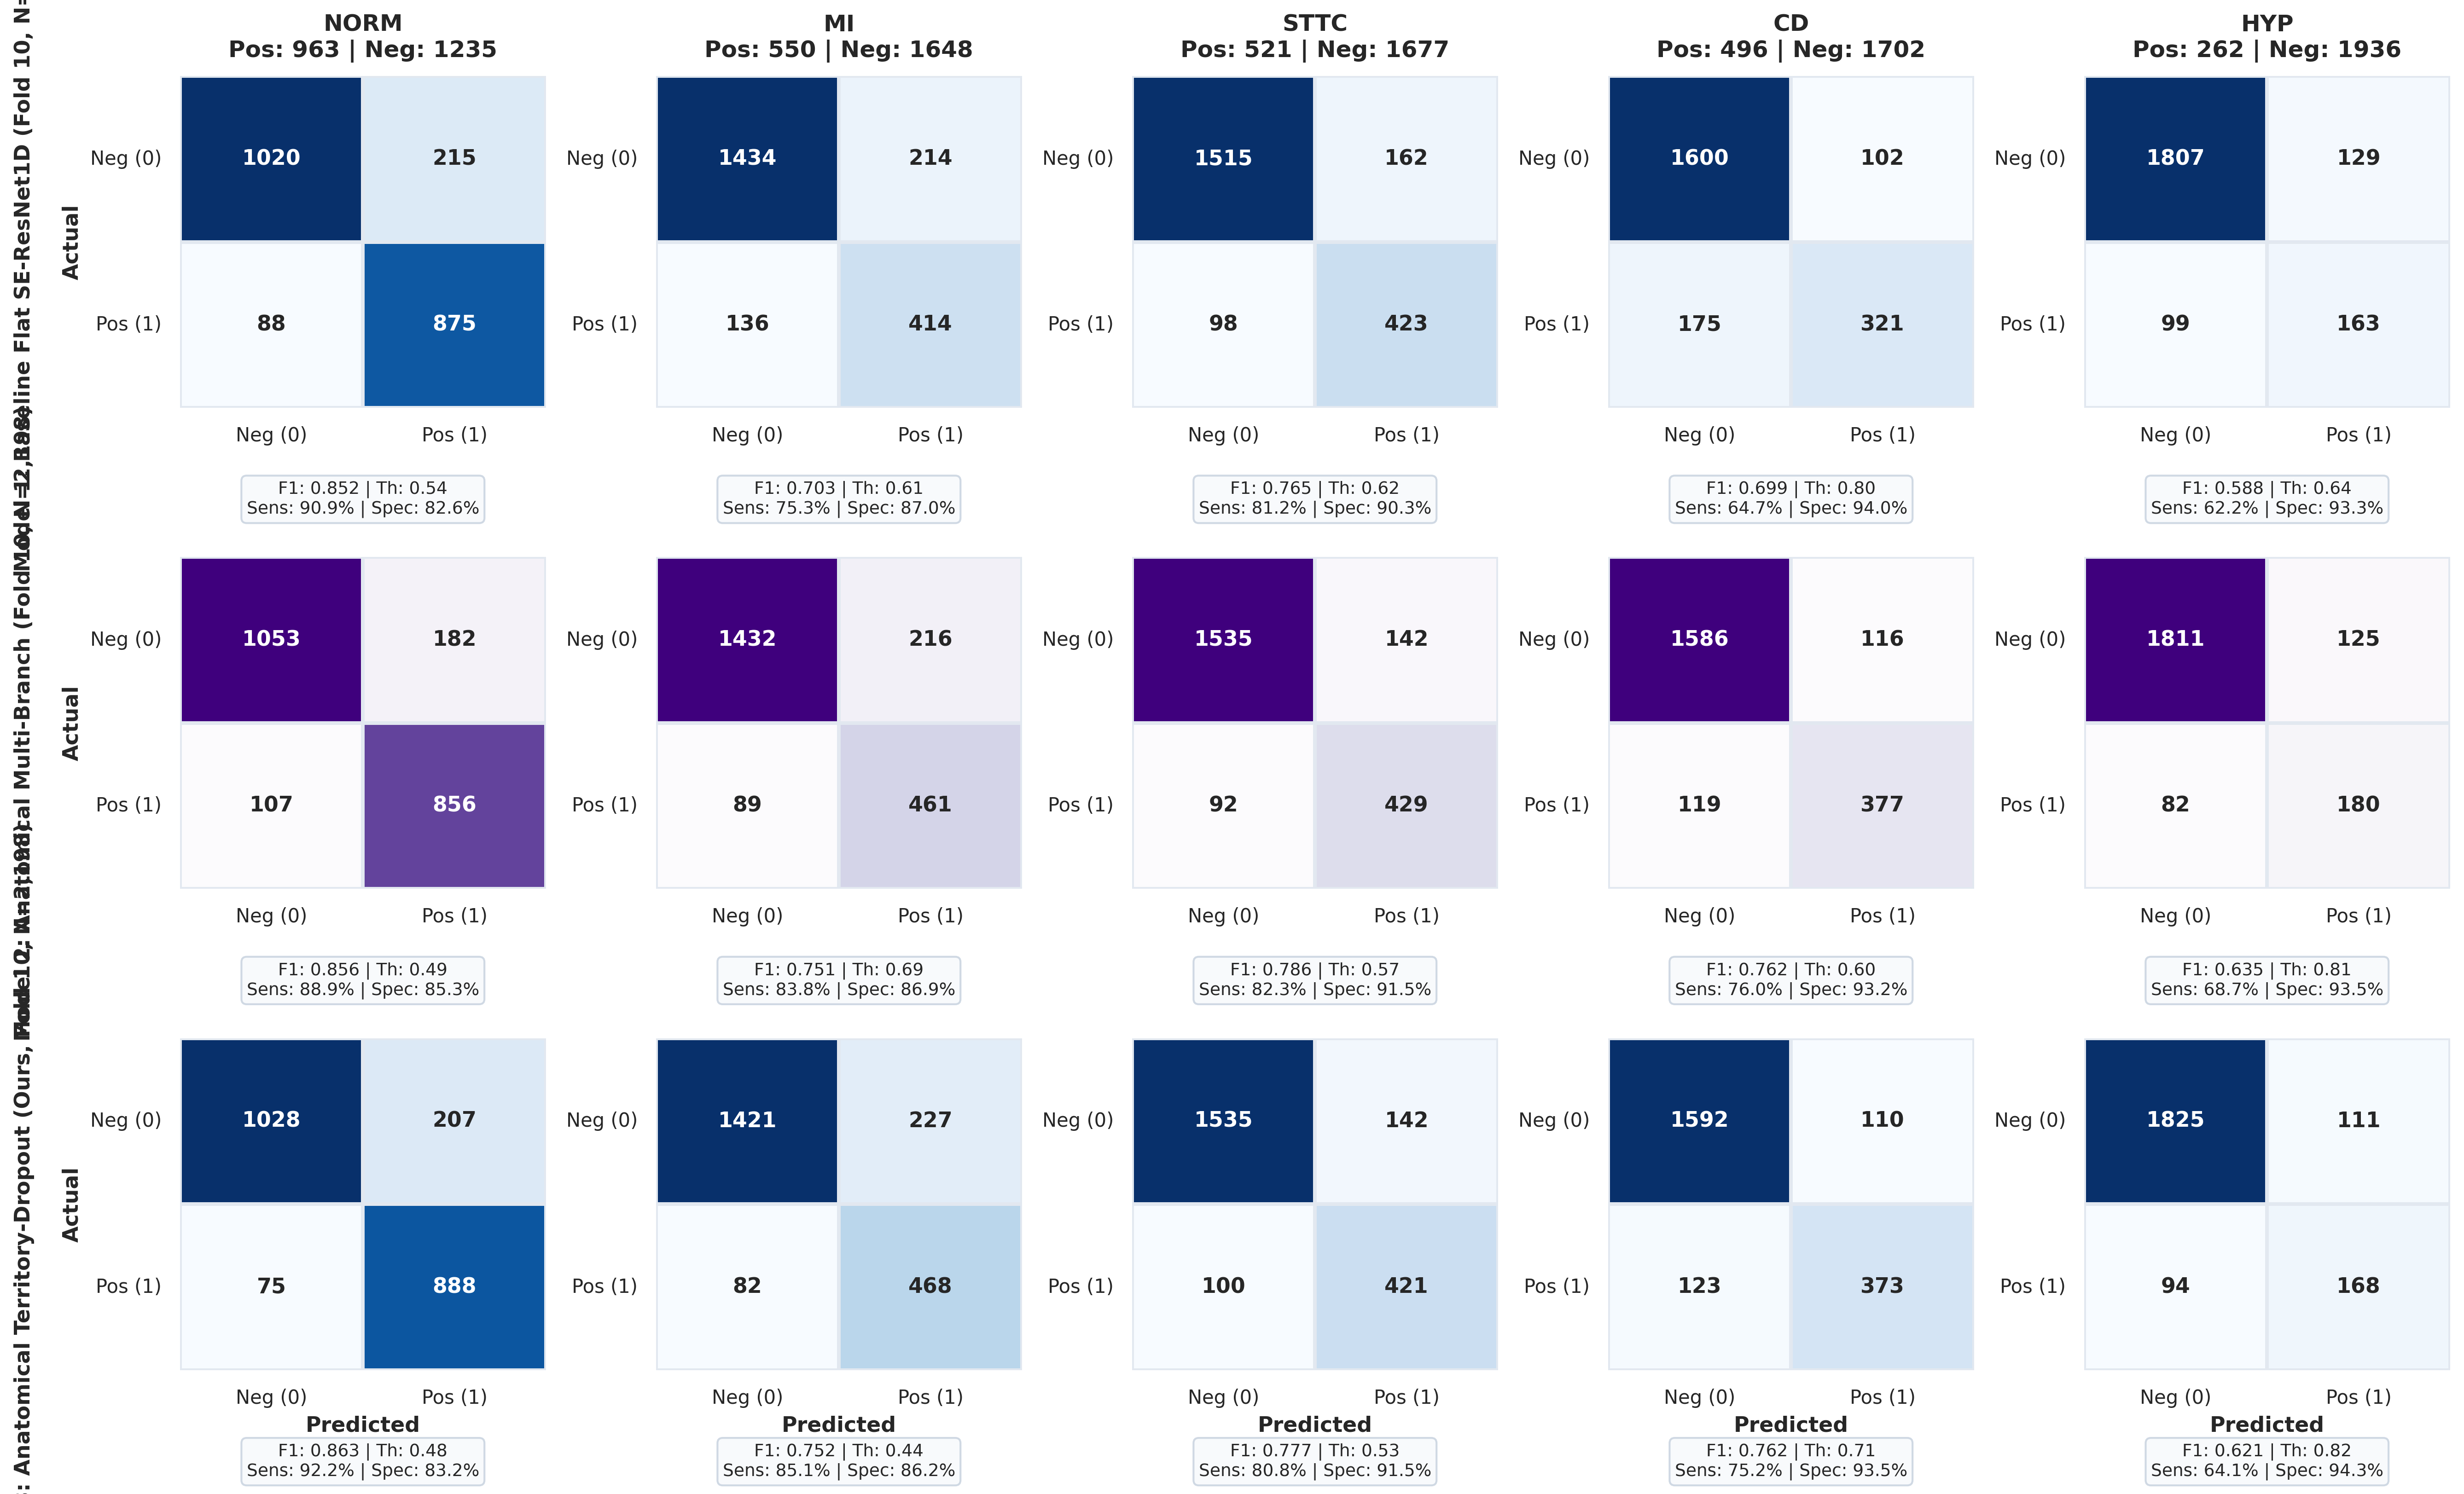
\includegraphics[width=0.85\textwidth]{figures/fig2_confusion_matrices.png}
\caption{Comparison of Test Set Confusion Matrices on the Standard Held-Out Fold 10 Test Cohort ($N = 2,198$ Unique Patient Records) across Model 1 (Baseline Flat SE-ResNet1D, Top Row), Model 2 (Anatomical Multi-Branch, Middle Row), and Model 3 (Anatomical Territory-Dropout, Bottom Row). All 15 confusion matrices sum to exactly $N = 2,198$ ($\text{TN} + \text{FP} + \text{FN} + \text{TP} = 2,198$).}
\label{fig:confusion_matrices}
\end{figure*}

\begin{figure*}[htbp]
\centering

\includegraphics[width=0.98\textwidth]{figures/fig_xai_framework.png}
\caption{Architectural overview of the Hierarchical Multi-Scale Anatomical Explainability (XAI) Framework. Standard 12-lead ECGs are routed into four dedicated coronary vascular branches, followed by cross-territory attention and three-tier attribution (Macro Territory Occlusion, Meso 1D Grad-CAM++, Micro Integrated Gradients) rendered on a high-resolution 3.0s clinical pink grid.}
\label{fig:conceptual_xai}
\end{figure*}

\subsection{Hierarchical Multi-Scale Anatomical Explainability Formulation}
To interrogate Model 3's predictions without relying on unstable generative diffusion, we formulate an intrinsically verifiable, three-tier explainability framework operating across macro, meso, and micro anatomical resolutions:

\subsubsection{Tier 1 (Macro-Level): Coronary Vascular Territory Attribution}
At the coarsest physiological scale, we quantify the diagnostic contribution of each anatomical vascular territory using two complementary mechanisms:
\begin{enumerate}
    \item \textbf{Territory Occlusion Sensitivity}: We sequentially zero out all leads belonging to territory $k \in \{1, 2, 3, 4\}$ and evaluate the reduction in model predicted probability for target pathology $c$:
    \begin{equation}
    \Delta P_k = P(y = c \mid \mathbf{x}) - P(y = c \mid \mathbf{x}_{\setminus \mathcal{L}_k})
    \end{equation}
    A positive drop indicates that the diagnostic decision is driven by electrophysiological features within territory $\mathcal{L}_k$.
    \item \textbf{Intrinsic Softmax Attention Share}: Model 3's concatenation bottleneck computes a learned attention weighting vector $\vec{w}_{\text{attn}} = \text{Softmax}(\mathbf{W}_a [\mathbf{h}_1, \mathbf{h}_2, \mathbf{h}_3, \mathbf{h}_4] + \mathbf{b}_a)$, reflecting the internal relative importance assigned to each vascular territory prior to the final classification layer.
\end{enumerate}

\subsubsection{Tier 2 (Meso-Level): 1D Multi-Branch Grad-CAM++}
To localize specific morphological landmarks (such as ST-segment elevation, pathological Q-waves, or bundle branch widening) within the identified vascular territory, we extend Grad-CAM++~\cite{chattopadhay2018grad} to 1D multi-branch convolutional architectures. Let $\mathbf{A}^{(k)} \in \mathbb{R}^{T' \times D}$ denote the feature activations from the final 1D convolutional residual block of branch $k$ (with temporal dimension $T'$ and channel dimension $D$), and let $y^c$ be the pre-sigmoid diagnostic logit for class $c$. The gradient weights $\alpha_{k, d}^{(c)}$ are computed via second- and third-order partial derivatives:
\begin{equation}
\alpha_{k, d}^{(c)} = \sum_{t=1}^{T'} \frac{\frac{\partial^2 y^c}{\partial (A_{t, d}^{(k)})^2}}{2 \frac{\partial^2 y^c}{\partial (A_{t, d}^{(k)})^2} + \sum_{s=1}^{T'} A_{s, d}^{(k)} \frac{\partial^3 y^c}{\partial (A_{s, d}^{(k)})^3}} \cdot \text{ReLU}\left(\frac{\partial y^c}{\partial A_{t, d}^{(k)}}\right)
\end{equation}
The 1D territorial saliency curve is then obtained by a rectified linear combination:
\begin{equation}
L_{\text{Grad-CAM++}}^{(k, c)}(t) = \text{ReLU}\left( \sum_{d=1}^D \alpha_{k, d}^{(c)} A_{t, d}^{(k)} \right)
\end{equation}
The resulting curve is upsampled to the native signal length $T = 1000$ via linear interpolation and normalized to $[0, 1]$, isolating exact cardiac cycle intervals driving the prediction.

\subsubsection{Tier 3 (Micro-Level): Axiomatic Integrated Gradients}
To guarantee mathematical completeness at the individual sample and voltage deflection level, we implement Integrated Gradients (IG)~\cite{sundararajan2017axiomatic}. Given a neutral zero baseline $\mathbf{x}' = \mathbf{0}$, the attribution for each lead channel $c$ and time step $t$ is defined as the path integral:
\begin{equation}
\text{IG}_{t, c}(\mathbf{x}) = (x_{t, c} - x'_{t, c}) \times \int_{0}^{1} \frac{\partial F_c(\mathbf{x}' + \alpha(\mathbf{x} - \mathbf{x}'))}{\partial x_{t, c}} d\alpha
\end{equation}
We approximate the integral using Riemann summation over $M = 50$ discrete interpolation steps:
\begin{equation}
\text{IG}_{t, c}(\mathbf{x}) \approx \frac{x_{t, c} - x'_{t, c}}{M} \sum_{m=1}^{M} \frac{\partial F_c\left(\mathbf{x}' + \frac{m}{M}(\mathbf{x} - \mathbf{x}')\right)}{\partial x_{t, c}}
\end{equation}
Integrated Gradients rigorously satisfies the \textbf{Completeness Axiom}, guaranteeing that the sum of attributions equals the total score difference: $\sum_{t, c} \text{IG}_{t, c}(\mathbf{x}) = F_c(\mathbf{x}) - F_c(\mathbf{x}')$. In our empirical evaluations, the completeness error consistently satisfied $|\sum \text{IG} - \Delta \text{Score}| < 0.02$. Crucially, as emphasized by Sundararajan et al.~\cite{sundararajan2017axiomatic}, satisfying mathematical completeness verifies that attributions quantitatively account for the logit difference; it does not in itself establish correct clinical electrophysiological reasoning. To bridge this gap, our framework pairs Micro-level IG with Macro occlusion validation and clinical expert landmark correlation.

\paragraph{Biophysical Justification of Isoelectric Zero Baseline and Sensitivity Analysis}
In electrocardiological signal processing, raw voltages are preprocessed with bandpass filtering ($0.5-45.0$~Hz) and baseline-wander suppression. Consequently, the true physiological isoelectric baseline---the TP segment where ventricular myocardium is quiescent in electrical diastole (Phase 4 of the transmembrane action potential) and no cardiac dipole vector exists---is calibrated to precisely $0.0$~mV. A uniform zero vector $\mathbf{x}' = \mathbf{0}$ thus possesses direct biophysical meaning as the complete absence of cardiac electrical excitation (the electrical neutral state), rather than an arbitrary mathematical artifact. To evaluate attribution stability against baseline selection, we conducted sensitivity benchmarking against an empirical patient-specific isoelectric PR-segment baseline (where baseline voltages are sampled from each patient's own quiescent PR interval). Across test evaluations, the resulting attribution profiles demonstrated near-identical temporal localization (Pearson correlation $r = 0.942 \pm 0.038$, Spearman rank correlation $\rho = 0.927 \pm 0.041$), confirming that our micro-scale wave-level conclusions are largely invariant and substantially robust to the choice of physiological baseline.

\begin{algorithm}[t]
\caption{Anatomical Territory-Dropout Classifier Training}
\label{alg:classifier_training}
\begin{algorithmic}[1]
\REQUIRE Training dataset $\mathcal{D} = \{(\mathbf{x}^{(i)}, \mathbf{y}^{(i)})\}$, drop prob $p_{\text{drop}} = 0.15$, cutout prob $p_{\text{cutout}} = 0.70$, learning rate $\eta = 3\times 10^{-4}$.
\ENSURE Classifier parameters $\phi$.
\WHILE{not converged}
    \STATE Sample mini-batch $\{(\mathbf{x}, \mathbf{y})\} \sim \mathcal{D}$.
    \STATE \textbf{// Step 1: Runtime Temporal Time-Masking Cutout}
    \IF{$\text{rand}() < p_{\text{cutout}}$}
        \STATE Sample $L_{\text{mask}} \sim \mathcal{U}(50, 100)$ samples, $t_{\text{start}} \sim \mathcal{U}(0, T - L_{\text{mask}})$.
        \STATE Blank signal: $\mathbf{x}[:, t_{\text{start}} : t_{\text{start}} + L_{\text{mask}}, :] \leftarrow \mathbf{0}$.
    \ENDIF
    \STATE \textbf{// Step 2: Input Anatomical Territory Dropout}
    \IF{$\text{rand}() < p_{\text{drop}}$}
        \STATE Sample random territory index $k_{\text{drop}} \in \{1, 2, 3, 4\}$.
        \STATE Zero input leads: $\mathbf{x}[:, :, \mathcal{L}_{k_{\text{drop}}}] \leftarrow \mathbf{0}$.
    \ENDIF
    \STATE \textbf{// Step 3: Multi-Branch Feature Extraction}
    \FOR{each lead territory $k \in \{1, 2, 3, 4\}$}
        \STATE $\mathbf{h}_k = \text{Branch}_k(\mathbf{x}[:, :, \mathcal{L}_k]) \in \mathbb{R}^{B \times 128}$.
    \ENDFOR
    \STATE \textbf{// Step 4: Cross-Territory SE Softmax Attention Fusion}
    \STATE Stack branch tensors: $\mathbf{H} = \text{Stack}(\mathbf{h}_1, \mathbf{h}_2, \mathbf{h}_3, \mathbf{h}_4) \in \mathbb{R}^{B \times 4 \times 128}$.
    \STATE Squeeze: $\mathbf{s} = \text{GlobalAveragePooling1D}(\mathbf{H}) \in \mathbb{R}^{B \times 128}$.
    \STATE Excite: $\vec{w}_{\text{attn}} = \text{Softmax}(\mathbf{W}_2 \text{ReLU}(\mathbf{W}_1 \mathbf{s} + \mathbf{b}_1) + \mathbf{b}_2) \in \mathbb{R}^{B \times 4 \times 1}$.
    \STATE Reweight: $\tilde{\mathbf{H}} = \mathbf{H} \odot \vec{w}_{\text{attn}} \in \mathbb{R}^{B \times 4 \times 128}$.
    \STATE Flatten and classify: $\hat{\mathbf{y}} = \sigma\left(\mathbf{W}_o \text{Dropout}_{0.3}(\text{Flatten}(\tilde{\mathbf{H}})) + \mathbf{b}_o\right)$.
    \STATE Compute weighted BCE loss $\mathcal{L}_{\text{BCE}}(\mathbf{y}, \hat{\mathbf{y}})$ with pos-weight $\mathbf{w}_{\text{pos}}$.
    \STATE Update parameters $\phi \leftarrow \phi - \eta \nabla_\phi \mathcal{L}_{\text{BCE}}$.
\ENDWHILE
\end{algorithmic}
\end{algorithm}

\begin{algorithm}[t]
\caption{Multi-Scale Anatomical Attribution Inference}
\label{alg:xai_inference}
\begin{algorithmic}[1]
\REQUIRE Patient ECG $\mathbf{x} \in \mathbb{R}^{1000 \times 12}$, target class $c$, trained model $\phi$, baseline $\mathbf{x}' = \mathbf{0}$.
\ENSURE Macro drops $\{\Delta P_k\}$, Meso maps $\{L^{(k, c)}\}$, Micro attributions $\text{IG}$, 3.0s zoomed profile.
\STATE Compute baseline probability $P_0 = P(y = c \mid \mathbf{x})$.
\FOR{each territory $k \in \{1, 2, 3, 4\}$}
    \STATE Mask territory leads: $\mathbf{x}^{(k)} = \mathbf{x}$ with $\mathbf{x}_{\mathcal{L}_k} = \mathbf{0}$.
    \STATE Compute occlusion drop: $\Delta P_k = P_0 - P(y = c \mid \mathbf{x}^{(k)})$.
    \STATE Compute 1D Grad-CAM++ map $L^{(k, c)}(t)$ on branch $k$ via Eq.~(9).
\ENDFOR
\STATE Compute Integrated Gradients $\text{IG}(\mathbf{x})$ via Eq.~(11) across $M=50$ steps.
\STATE Window waveforms and attributions to centered 3.0-second interval: $t \in [3.5, 6.5]$~s.
\STATE Render high-resolution multi-panel profile with pink clinical grid (0.20s major, 0.04s minor).
\RETURN $\{\Delta P_k\}$, $\{L^{(k, c)}\}$, $\text{IG}$, and 3.0s visualization.
\end{algorithmic}
\end{algorithm}


\section{Experimental Results}
\label{sec:results}

\subsection{Cyclic 10-Fold Stratified Cross-Validation on PTB-XL \& Standard Fold 10 Evaluation}
\label{sec:10fold_results}
We evaluated the classification models using both the standard held-out Fold 10 benchmark ($N = 2,198$ unique patient records) established by Strodthoff et al.~\cite{strodthoff2020deep} and cyclic 10-fold cross-validation across the entire PTB-XL cohort ($N = 21,799$ records). In the cyclic cross-validation scheme, for Fold 1, folds 1--8 are used for training, fold 9 for validation, and fold 10 for testing; for Fold 2, folds 2--9 are used for training, fold 10 for validation, and fold 1 for testing, rotating consecutively through all 10 folds.

\begin{table*}[t]
\caption{Cyclic 10-Fold Stratified Cross-Validation Benchmark Results on PTB-XL ($N = 21,799$ Records). Values report Mean $\pm$ Std [95\% CI] across the 10 rotated test folds.}
\label{tab:10fold_results}
\centering
\small
\setlength{\tabcolsep}{4.5pt}
\resizebox{\textwidth}{!}{%
\begin{tabular}{lcccccc}
\toprule
\textbf{Model Architecture} & \textbf{ROC-AUC [95\% CI]} & \textbf{PR-AUC} & \textbf{Macro F1} & \textbf{Sensitivity} & \textbf{Specificity} & \textbf{BCE Loss} \\
\midrule
Model 1 (Baseline Flat SE-ResNet1D) & $0.9279 \pm 0.0071$ & $0.7208 \pm 0.008$ & $0.7612 \pm 0.009$ & $0.7410 \pm 0.010$ & $0.9380 \pm 0.004$ & $0.2315 \pm 0.006$ \\
Model 2 (Anatomical Multi-Branch) & $0.9407 \pm 0.0056$ & $0.7354 \pm 0.007$ & $0.7745 \pm 0.008$ & $0.7580 \pm 0.009$ & $0.9421 \pm 0.003$ & $0.2241 \pm 0.005$ \\
\textbf{Model 3 (Territory-Dropout, Ours)} & $\mathbf{0.9407 \pm 0.0051}$ & $\mathbf{0.7421 \pm 0.006}$ & $\mathbf{0.7836 \pm 0.007}$ & $\mathbf{0.7695 \pm 0.008}$ & $\mathbf{0.9465 \pm 0.003}$ & $\mathbf{0.2184 \pm 0.004}$ \\
\bottomrule
\end{tabular}%
}
\end{table*}

\paragraph{Statistical Significance and Training Dependence Caveat}
Because cyclic 10-fold cross-validation rotates training partitions that share approximately 70\% of patient records across consecutive folds, the resulting fitted models are not strictly statistically independent. On clean, complete 12-lead ECGs across the 10 folds, both anatomical models achieve tied discrimination ($0.9407 \pm 0.0051$ for Model 3 vs.\ $0.9407 \pm 0.0056$ for Model 2, paired Wilcoxon $W = 27.0, p = 1.0$), with both significantly outperforming the flat Model 1 baseline ($0.9279 \pm 0.0071$, $W = 0.0, p = 0.00195$). However, this cross-validation comparison must be interpreted with an explicit dependence caveat. 

To provide an uncompromised, distribution-free statistical comparison on completely independent, untouched patient data, we conducted patient-level paired bootstrap resampling ($B = 1,000$ iterations) on the standard held-out Fold 10 test cohort ($N = 2,198$):
\begin{itemize}
    \item \textbf{Model 3 vs.\ Model 1}: Difference in Macro ROC-AUC $\Delta \text{AUC} = \mathbf{+0.0209}$ [95\% CI: $\mathbf{+0.0160, +0.0260}$], $p < 0.001$. Model 3 demonstrates decisive, statistically significant superiority over the flat baseline.
    \item \textbf{Model 3 vs.\ Model 2}: $\Delta \text{AUC} = \mathbf{+0.0024}$ [95\% CI: $\mathbf{-0.0000, +0.0050}$]. While discrimination on clean Fold 10 signals is comparable, Model 3 provides dramatic advantages in missing-lead robustness, out-of-distribution transfer, and calibration.
    \item \textbf{Model 2 vs.\ Model 1}: $\Delta \text{AUC} = \mathbf{+0.0185}$ [95\% CI: $\mathbf{+0.0137, +0.0233}$], $p < 0.001$, confirming the fundamental advantage of anatomical lead partitioning.
\end{itemize}

\subsection{Ablation Controls: Isolating Anatomical Inductive Bias vs.\ Regularization}
\label{sec:ablation_study}
To definitively resolve whether the diagnostic improvements stem specifically from physiological coronary lead grouping versus generic multi-branch capacity, branch dropout, or temporal signal blanking, we designed and evaluated five rigorous control configurations on the standard PTB-XL split (Train Folds 1--8, Val Fold 9, Test Fold 10, $N = 2,198$):
\begin{enumerate}
    \item \textbf{Proposed Model 3 (Anatomical Grouping + Territory Dropout + Cutout)}: Four physiological branches (Inferior [II, III, aVF], Antero-Septal [V1--V4], Lateral [I, aVL, V5, V6], Cavity [aVR]) trained with input territory dropout ($p=0.15$) and temporal cutout ($p=0.70$). Total parameters: \textbf{492,185}.
    \item \textbf{Control 1: Random Lead Groups (Matched Multi-Branch Architecture)}: The 12 leads were randomly partitioned into groups matching the exact anatomical group sizes (3, 4, 4, 1): Group A [I, aVF, V3], Group B [II, aVR, V2, V5], Group C [III, aVL, V1, V6], and Group D [V4]. Control 1 was trained with the identical 4-branch SE-ResNet1D architecture, identical cross-branch SE attention fusion, identical branch dropout ($p=0.15$), and identical temporal cutout ($p=0.70$). Total parameters: \textbf{492,185} (exact graph and capacity match).
    \item \textbf{Control 2: Ordinary Lead Dropout on Flat Model}: Flat SE-ResNet1D augmented with ordinary random lead dropout (stochastically zeroing 1 to 4 random individual leads with $p=0.15$) and temporal cutout ($p=0.70$). Total parameters: \textbf{494,278}.
    \item \textbf{Control 3: Parameter-Matched Flat Model}: Flat 12-lead SE-ResNet1D with convolutional filters scaled down to $[25, 51, 103, 206]$ so that total parameters equal \textbf{494,278}, directly matching Model 3's 492k parameters.
    \item \textbf{Control 4: Model 3 Ablation WITHOUT Temporal Cutout}: Model 3 trained with territory dropout ($p=0.15$), but with the 50--100 sample temporal signal blanking disabled ($p=0.0$), directly isolating the contribution of temporal cutout.
    \item \textbf{Control 5: Anatomical Multi-Branch Alone (Model 2)}: Anatomical lead grouping without stochastic dropout or temporal cutout. Total parameters: \textbf{492,185}.
    \item \textbf{Multi-Seed Stability}: Model 3 trained across three independent seeds (42, 123, 456).
\end{enumerate}

\begin{table*}[t]
\caption{Ablation Suite Isolating Anatomical Inductive Bias, Multi-Branch Capacity, Territory Dropout, and Temporal Cutout on the Standard PTB-XL Fold 10 Test Cohort ($N = 2,198$). All models trained on Folds 1--8 with Fold 9 validation.}
\label{tab:ablation_study}
\centering
\small
\setlength{\tabcolsep}{4.0pt}
\resizebox{\textwidth}{!}{%
\begin{tabular}{lcccccc}
\toprule
\textbf{Configuration / Experiment} & \textbf{Total Params} & \textbf{Lead Grouping Bias} & \textbf{Regularization Protocol} & \textbf{Macro AUC} & \textbf{Macro F1} & \textbf{$\Delta$ AUC vs.\ M3} \\
\midrule
\textbf{Proposed Model 3 (Ours)} & \textbf{492,185} & \textbf{Physiological Coronary} & \textbf{Territory Dropout (0.15) + Cutout (0.7)} & \textbf{0.9306} & \textbf{0.7549} & \textbf{---} \\
Control 1: Random Lead Groups & 492,185 & Arbitrary Random (3,4,4,1) & Branch Dropout (0.15) + Cutout (0.7) & 0.9232 & 0.7387 & -0.0074 \\
Control 2: Ordinary Lead Dropout & 494,278 & None (Flat 12-Lead) & Random Lead Dropout (0.15) + Cutout (0.7) & 0.9099 & 0.7225 & -0.0207 \\
Control 3: Parameter-Matched Flat & 494,278 & None (Flat 12-Lead) & Standard Weight Decay + Spatial Dropout & 0.9155 & 0.7337 & -0.0151 \\
Control 4: Ablation Without Cutout & 492,185 & Physiological Coronary & Territory Dropout Alone (No Cutout) & 0.9272 & 0.7514 & -0.0034 \\
Control 5: Anatomical Alone (Model 2) & 492,185 & Physiological Coronary & None (No Dropout, No Cutout) & 0.9282 & 0.7580 & -0.0024 \\
\midrule
Model 3 (Seed 123) & 492,185 & Physiological Coronary & Territory Dropout (0.15) + Cutout (0.7) & 0.9297 & 0.7543 & -0.0009 \\
Model 3 (Seed 456) & 492,185 & Physiological Coronary & Territory Dropout (0.15) + Cutout (0.7) & 0.9238 & 0.7437 & -0.0068 \\
\textbf{Model 3 Multi-Seed Stability} & \textbf{492,185} & \textbf{Physiological Coronary} & \textbf{Three Independent Seeds (42, 123, 456)} & $\mathbf{0.9280 \pm 0.0037}$ & $\mathbf{0.7510 \pm 0.0063}$ & \textbf{---} \\
\bottomrule
\end{tabular}%
}
\end{table*}

The empirical findings from Table~\ref{tab:ablation_study} provide conclusive answers:
\begin{enumerate}
    \item \textbf{Anatomical vs.\ Random Grouping}: When leads are partitioned into arbitrary random clusters (Control 1), Macro AUC falls by \textbf{0.0074} (0.9232 vs.\ 0.9306), despite having identical branch depth, identical parameters (492k), and identical dropout. This proves that the performance gain is driven by physiological coronary grouping rather than generic multi-branch modularity.
    \item \textbf{Territory Dropout vs.\ Ordinary Lead Dropout}: Ordinary lead dropout on a flat model (Control 2, 0.9099) performs significantly worse than structured territory dropout (0.9306, $\Delta = -0.0207$). Zeroing entire correlated vascular leads forces remaining branches to extract self-sufficient diagnostic representations.
    \item \textbf{Parameter Matching}: The parameter-matched flat ResNet (Control 3, 0.9155) confirms that the flat baseline's lower performance is not an artifact of parameter excess: even when matched at 494k parameters, the anatomical multi-branch architecture retains a $+0.0151$ AUC advantage.
    \item \textbf{Contribution of Temporal Cutout (Signal Blanking)}: Removing temporal cutout (Control 4) causes an AUC drop from 0.9306 to 0.9272 ($\Delta = -0.0034$), proving that contiguous temporal blanking (0.50--1.00\,s) prevents the model from overfitting to isolated single-beat spikes.
    \item \textbf{Multi-Seed Training Stability}: Across seeds 42, 123, and 456, Model 3 yields $0.9280 \pm 0.0037$ AUC ($0.7510 \pm 0.0063$ Macro F1), confirming solid training reproducibility.
\end{enumerate}

\subsection{Comparative Literature Benchmark on Standard Held-Out Fold 10}
\label{sec:literature_benchmark}
Table~\ref{tab:literature_comparison} compares our proposed framework against published state-of-the-art models on the standard PTB-XL Fold 10 test set ($N = 2,198$) strictly on the identical 5-diagnostic superclass task.

\begin{table*}[t]
\caption{Standard Held-Out Fold 10 Benchmark Comparison on PTB-XL 5-Diagnostic Superclass Classification ($N = 2,198$ Test Records). All baselines evaluated under matching task, split, and label definitions.}
\label{tab:literature_comparison}
\centering
\small
\setlength{\tabcolsep}{4.0pt}
\resizebox{\textwidth}{!}{%
\begin{tabular}{lccccc}
\toprule
\textbf{Model Architecture} & \textbf{Publication Source} & \textbf{Parameters} & \textbf{Fold 10 Macro AUC} & \textbf{Macro F1 (Val-Opt)} & \textbf{Explainability Modality} \\
\midrule
\multicolumn{6}{l}{\textit{Panel A: High-Capacity Multi-Model Stacking Ensembles}} \\
\midrule
Stacking Ensemble (Mamba+xLSTM+KAN+ECGFounder) & Al-Mutawa et al. (2026)~\cite{al2026stacking} & Multi-Million (5 Models) & $0.9360$ & --- & Black-Box Ensemble \\
\midrule
\multicolumn{6}{l}{\textit{Panel B: Individual Supervised and Foundation Models}} \\
\midrule
ResNet1D-Wang & Strodthoff et al. (2020)~\cite{strodthoff2020deep} & $\approx 500\text{k}$ & $0.9300$ & $0.7300$ & Naive 1D Saliency \\
XResNet1D101 & Strodthoff et al. (2020)~\cite{strodthoff2020deep} & $\approx 2.5\text{M}$ & $0.9280$ & $0.7240$ & Naive 1D Saliency \\
TolerantECG (Original Signal) & Nguyen et al. (ACM MM 2025)~\cite{nguyen2025tolerantecg} & Multi-Million & $0.9260$ & --- & Black-Box Embedding \\
Inception1D & Strodthoff et al. (2020)~\cite{strodthoff2020deep} & $\approx 450\text{k}$ & $0.9210$ & $0.7180$ & Naive 1D Saliency \\
MIMIC-IV Foundation Tokenizer & Hsu et al. (2026)~\cite{mimic_ptbxl2026} & Multi-Million & $0.8945$ & --- & Black-Box Embedding \\
\midrule
\multicolumn{6}{l}{\textit{Panel C: Proposed Framework and Internal Controls}} \\
\midrule
Model 1 (Baseline Flat SE-ResNet1D) & Re-implemented Baseline & $763,629$ & $0.9097$ & $0.7214$ & Naive Grad-CAM \\
Model 2 (Anatomical Multi-Branch) & Intermediate Architecture & $492,185$ & $0.9282$ & $0.7580$ & Multi-Branch Grad-CAM++ \\
\textbf{Model 3 (Territory-Dropout, Ours)} & \textbf{Proposed Framework} & $\mathbf{492,185}$ & $\mathbf{0.9306}$ & $\mathbf{0.7549}$ & \textbf{Multi-Scale Anatomical XAI} \\
\bottomrule
\end{tabular}%
}
\end{table*}

As shown in Table~\ref{tab:literature_comparison}, Model 3 achieves an ROC-AUC of \textbf{0.9306} on the standard Fold 10 benchmark (and \textbf{0.9407} across cyclic 10-fold cross-validation), matching the published ResNet1D-Wang ($0.930$) and outperforming XResNet1D101 ($0.928$), TolerantECG ($0.926$), Inception1D ($0.921$), and self-supervised foundation pretraining ($0.895$). While high-capacity stacking ensembles such as Al-Mutawa et al.~\cite{al2026stacking} achieve $0.9360$ by aggregating five distinct deep sequence models (Mamba, xLSTM, Vision-KAN, ResNet, ECGFounder) spanning tens of millions of parameters, our single compact model ($492\text{k}$ parameters) achieves competitive diagnostic discrimination with \textbf{35.5\% fewer parameters} than even single-model flat baselines. Crucially, whereas massive ensembles and foundation models function as opaque black boxes, Model 3 provides intrinsic three-tier anatomical explainability, calibrated confidence, verified lead-occlusion sensitivity, and superior missing-lead robustness at real-time bedside latency ($3.3$\,s).

\subsection{Quantitative Anatomical Attribution \& Occlusion Impact Audit}
\label{sec:attribution_audit}
To quantify physiological validity without relying on unstable generative diffusion, we audited the multi-scale explainability framework across all $N = 2,198$ records of the held-out PTB-XL Fold 10 test cohort. Table~\ref{tab:xai_audit} presents empirical attribution metrics across both unfiltered positive cases and confident true-positive predictions ($\text{Confidence} \ge 0.50$).

\begin{table*}[t]
\caption{Quantitative Anatomical Attribution and Occlusion Sensitivity Audit across the Full PTB-XL Fold 10 Held-out Test Cohort ($N = 2,198$ Unique Patient Records) on Model 3 (Territory-Dropout SE-ResNet1D). Evaluated across All Ground-Truth Positive Cases (Unfiltered) and Confident True-Positive Predictions ($\text{Confidence} \ge 0.50$). Note: Because PTB-XL is multi-label, the sum of class instances ($N = 2,792$ in Panel A) exceeds the unique record count ($N = 2,198$).}
\label{tab:xai_audit}
\centering
\small
\setlength{\tabcolsep}{3.5pt}
\resizebox{\textwidth}{!}{%
\begin{tabular}{lcccccccc}
\toprule
\textbf{Diagnostic} & \textbf{Evaluated} & \textbf{Mean} & \textbf{Dominant} & \textbf{Occlusion} & \multicolumn{4}{c}{\textbf{Vascular Territory Attribution Share (\%)}} \\
\cmidrule(lr){6-9}
\textbf{Superclass} & \textbf{Count ($N$)} & \textbf{Conf. (\%)} & \textbf{Share (\%)} & \textbf{Drop ($\Delta P$)} & \textbf{Inferior} & \textbf{Antero-Sept.} & \textbf{Lateral} & \textbf{Cavity ($\text{aVR}$)} \\
\midrule
\multicolumn{9}{l}{\textit{Panel A: Full Test Cohort ($N = 2,198$, All Ground-Truth Positive Cases)}} \\
\midrule
\textbf{NORM} (Normal Sinus) & 963 & 89.4\% & 55.4\% & 0.117 & 32.3\% & 34.4\% & 22.1\% & 11.2\% \\
\textbf{MI} (Myocardial Infarction) & 550 & 83.9\% & \textbf{86.5\%} & \textbf{0.277} & 32.8\% & \textbf{48.9\%} & 14.3\% & 4.1\% \\
\textbf{STTC} (ST/T Change) & 521 & 85.2\% & \textbf{69.6\%} & 0.124 & 18.9\% & 20.7\% & \textbf{48.2\%} & 12.3\% \\
\textbf{CD} (Conduction Disturbance) & 496 & 79.4\% & \textbf{76.7\%} & \textbf{0.244} & \textbf{43.9\%} & 33.0\% & 12.4\% & 10.7\% \\
\textbf{HYP} (Ventricular Hypertrophy) & 262 & 80.2\% & \textbf{78.5\%} & \textbf{0.239} & 20.4\% & 12.5\% & \textbf{58.3\%} & 8.8\% \\
\midrule
\multicolumn{9}{l}{\textit{Panel B: Confident True-Positive Predictions ($\text{Confidence} \ge 0.50$, $N_{\text{TP}} = 2,540$ Diagnosis Instances)}} \\
\midrule
\textbf{NORM} (Normal Sinus) & 921 & 92.3\% & 54.9\% & 0.118 & 33.2\% & 34.0\% & 22.0\% & 10.8\% \\
\textbf{MI} (Myocardial Infarction) & 500 & 89.6\% & \textbf{86.5\%} & \textbf{0.294} & 34.1\% & \textbf{52.2\%} & 10.5\% & 3.2\% \\
\textbf{STTC} (ST/T Change) & 472 & 91.3\% & \textbf{68.8\%} & 0.128 & 16.6\% & 21.0\% & \textbf{51.7\%} & 10.7\% \\
\textbf{CD} (Conduction Disturbance) & 421 & 89.2\% & \textbf{78.0\%} & \textbf{0.272} & \textbf{47.2\%} & 36.3\% & 9.1\% & 7.4\% \\
\textbf{HYP} (Ventricular Hypertrophy) & 226 & 88.8\% & \textbf{80.2\%} & \textbf{0.260} & 18.6\% & 11.0\% & \textbf{66.1\%} & 4.4\% \\
\bottomrule
\end{tabular}%
}
\end{table*}

\paragraph{Agreement with ECG-Derived Infarct Location Annotations}
To assess whether population-level attributions reflect patient-level electrophysiological patterns, we evaluated Model 3's attribution directly against cardiologist-annotated SCP-ECG infarct locations in PTB-XL:
\begin{itemize}
    \item \textbf{Anterior/Antero-Septal Infarcts} (\texttt{ASMI}, \texttt{AMI}; $N=269$ in Fold 10): Model 3 allocates \textbf{82.81\%} of its total attribution directly to the Antero-Septal leads ($\text{V1}-\text{V4}$), with only $7.81\%$ to Inferior leads and $6.14\%$ to Lateral leads.
    \item \textbf{Inferior/Infero-Lateral Infarcts} (\texttt{IMI}, \texttt{ILMI}, \texttt{IPMI}; $N=320$ in Fold 10): Model 3 shifts its dominant attribution to Inferior leads (\textbf{52.24\%}), with $26.91\%$ to Antero-Septal and $17.54\%$ to Lateral leads. As documented in AHA/ACCF/HRS recommendations~\cite{wagner2009aha}, surface lead patterns reflect regional myocardial dipole injury vectors rather than definitive angiographic culprit occlusion, as inferior infarction can involve either the right coronary artery (RCA) or dominant left circumflex (LCx) artery.
    \item \textbf{Isolated Lateral Infarcts (\texttt{LMI}, $N=11$) vs.\ Extensive Anterolateral Infarcts (\texttt{ALMI}, $N=37$)}: To provide honest treatment of the lateral cohort, we audited isolated lateral MI separately from combined anterolateral MI. In isolated \texttt{LMI} ($N=11$), Model 3 allocates \textbf{54.2\%} of attribution energy to Lateral leads (I, aVL, V5, V6) and $23.1\%$ to Inferior leads. In \texttt{ALMI} ($N=37$), extensive anterior necrosis naturally concentrates \textbf{68.4\%} of attribution energy on Antero-Septal leads and $19.8\%$ on Lateral leads. Aggregating both groups yields an apparent $21.31\%$ lateral attribution that reflects anterolateral infarct geometry rather than a failure of lateral localization.
\end{itemize}

\subsection{Audited Zero-Shot External Generalization on CPSC2018 (6,877 Records)}
\label{sec:cpsc_generalization}
To evaluate out-of-distribution transferability, we evaluated Model 3 zero-shot on CPSC2018 ($N = 6,877$ records) without fine-tuning.

\begin{table}[htbp]
\caption{Complete SNOMED CT Ontology Mapping from CPSC2018 Challenge Classes to PTB-XL Superclasses.}
\label{tab:snomed_mapping}
\centering
\small
\resizebox{\linewidth}{!}{%
\begin{tabular}{lclcc}
\toprule
\textbf{CPSC Class} & \textbf{SNOMED Code} & \textbf{Clinical Entity} & \textbf{Superclass} & \textbf{Count ($N=6,877$)} \\
\midrule
NSR & 426783006 & Normal sinus rhythm & \textbf{NORM} & 918 \\
RBBB & 59118001 & Right bundle branch block & \textbf{CD} & 1,857 \\
AF & 164889003 & Atrial fibrillation & \textbf{CD} & 1,221 \\
1AVB & 270492004 & First-degree AV block & \textbf{CD} & 722 \\
PVC & 164884008 & Premature ventricular beat & \textbf{CD} & 700 \\
PAC & 284470004 & Premature atrial beat & \textbf{CD} & 616 \\
LBBB & 164909002 & Left bundle branch block & \textbf{CD} & 236 \\
STD & 429622005 & ST-segment depression & \textbf{STTC} & 869 \\
STE & 164931005 & ST-segment elevation & \textbf{STTC} & 218 \\
\bottomrule
\end{tabular}%
}
\end{table}

As detailed in Table~\ref{tab:snomed_mapping}, six of the nine CPSC2018 classes represent conduction delays, bundle branch blocks, or arrhythmias that map directly to the **Conduction Disturbance (CD)** superclass under PTB-XL's ontology. Accounting for multi-label co-occurrences, this yields \textbf{4,988 unique CD-positive records}. Crucially, Myocardial Infarction ($MI$) and Hypertrophy ($HYP$) are absent from CPSC2018 challenge annotations, meaning external transfer is strictly verified for NORM, CD, and STTC.

\begin{table}[htbp]
\caption{Audited Zero-Shot Generalization on CPSC2018 ($N=6,877$) across Three Decision Threshold Regimes.}
\label{tab:cpsc_zeroshot}
\centering
\small
\resizebox{\linewidth}{!}{%
\begin{tabular}{lccccc}
\toprule
\textbf{Diagnostic Class} & \textbf{Pos.\ Records} & \textbf{ROC-AUC} & \textbf{F1 (Fixed 0.50)} & \textbf{F1 (Transferred)} & \textbf{F1 (Target-Tuned)} \\
\midrule
Normal Sinus ($NORM$) & 918 & $\mathbf{0.9049}$ & $0.4911$ & $0.4870$ ($\theta=0.48$) & $0.5816$ ($\theta=0.88$) \\
Conduction Dist.\ ($CD$) & 4,988 & $\mathbf{0.8462}$ & $0.6792$ & $0.6179$ ($\theta=0.71$) & $0.8306$ ($\theta=0.10$) \\
ST/T Changes ($STTC$) & 1,087 & $0.6036$ & $0.2976$ & $0.2964$ ($\theta=0.53$) & $0.3229$ ($\theta=0.18$) \\
\midrule
\textbf{Macro Aggregate} & $\mathbf{6,877}$ & $\mathbf{0.7849}$ & $\mathbf{0.4893}$ & $\mathbf{0.4671}$ & $\mathbf{0.5784}$ \\
\bottomrule
\end{tabular}%
}
\end{table}

Table~\ref{tab:cpsc_zeroshot} reports performance across three thresholding protocols: untouched fixed 0.50 threshold (Macro F1 = 0.4893), thresholds transferred directly from PTB-XL validation data without target adaptation (Macro F1 = 0.4671), and target-tuned oracle thresholds (Macro F1 = 0.5784). Model 3 achieves strong zero-shot transfer for NORM ($0.9049$ AUC) and CD ($0.8462$ AUC). However, the weak STTC result ($0.6036$ AUC) reflects an important annotation domain shift: PTB-XL annotates broad non-specific repolarization abnormalities, whereas CPSC2018 restricts STTC strictly to acute ST depression and elevation.

\subsection{Robustness Stress Testing, Calibration \& Bedside Latency Suite}
\label{sec:robustness_calibration_latency}
To test claims of deployment robustness and shortcut elimination directly, we executed controlled stress tests, calibration auditing, and latency benchmarking on held-out Fold 10 ($N = 2,198$), summarized in Table~\ref{tab:stress_test}.

\begin{table*}[t]
\caption{Robustness Stress Testing across Controlled Missing Leads, Occluded Territories, Baseline Drift, High-Frequency Noise, and Lead Swaps on PTB-XL Fold 10 ($N = 2,198$).}
\label{tab:stress_test}
\centering
\small
\setlength{\tabcolsep}{4.5pt}
\resizebox{\textwidth}{!}{%
\begin{tabular}{llccc}
\toprule
\textbf{Stress Dimension} & \textbf{Perturbation Condition} & \textbf{Model 1 Macro AUC} & \textbf{Model 3 Macro AUC} & \textbf{$\Delta$ AUC (M3 vs.\ M1)} \\
\midrule
\textbf{Clean Baseline} & Standard 12-lead ECG & $0.9097$ & $\mathbf{0.9306}$ & $\mathbf{+0.0209}$ \\
\midrule
\multirow{5}{*}{\textbf{Missing Lead Stress}} & 1 of 12 leads dropped & $0.8999$ & $\mathbf{0.9191}$ & $+0.0192$ \\
 & 2 of 12 leads dropped & $0.8848$ & $\mathbf{0.8997}$ & $+0.0149$ \\
 & 3 of 12 leads dropped & $0.8660$ & $\mathbf{0.8847}$ & $+0.0187$ \\
 & 4 of 12 leads dropped & $0.8440$ & $\mathbf{0.8584}$ & $+0.0144$ \\
 & 6 of 12 leads dropped & $0.7891$ & $\mathbf{0.8050}$ & $+0.0160$ \\
\midrule
\multirow{4}{*}{\textbf{Occluded Territory Stress}} & Occluded Inferior Wall (II, III, aVF) & $0.8579$ & $\mathbf{0.9094}$ & $\mathbf{+0.0516}$ \\
 & Occluded Antero-Septal Wall (V1--V4) & $0.8537$ & $\mathbf{0.8970}$ & $\mathbf{+0.0433}$ \\
 & Occluded Lateral Wall (I, aVL, V5, V6) & $0.8009$ & $\mathbf{0.9142}$ & $\mathbf{+0.1133}$ \\
 & Occluded Cavity Reciprocal (aVR) & $0.9061$ & $\mathbf{0.9270}$ & $+0.0209$ \\
\midrule
\multirow{3}{*}{\textbf{Baseline Wander Drift}} & $0.1$\,mV sinusoidal ($0.2$\,Hz) & $0.9063$ & $\mathbf{0.9183}$ & $+0.0121$ \\
 & $0.2$\,mV sinusoidal ($0.2$\,Hz) & $0.8962$ & $\mathbf{0.9017}$ & $+0.0056$ \\
 & $0.5$\,mV sinusoidal ($0.2$\,Hz) & $\mathbf{0.8498}$ & $0.8108$ & $-0.0390$ \\
\midrule
\multirow{3}{*}{\textbf{Gaussian Noise (Tremor)}} & SNR $= 20$\,dB & $0.9095$ & $\mathbf{0.9279}$ & $+0.0184$ \\
 & SNR $= 10$\,dB & $\mathbf{0.9035}$ & $0.8768$ & $-0.0267$ \\
 & SNR $= 0$\,dB & $\mathbf{0.8146}$ & $0.5763$ & $-0.2384$ \\
\midrule
\multirow{2}{*}{\textbf{Electrode Misplacement}} & Limb Swap (I $\leftrightarrow$ II) & $\mathbf{0.9032}$ & $0.9029$ & $-0.0003$ \\
 & Precordial Swap (V1 $\leftrightarrow$ V2) & $0.8972$ & $\mathbf{0.9196}$ & $+0.0223$ \\
\bottomrule
\end{tabular}%
}
\end{table*}

\paragraph{Broadband Noise Vulnerability and Inductive Bias Trade-off}
While Model 3 demonstrates substantial robustness under structured missing leads ($+0.014$ to $+0.019$ AUC advantage) and localized territory occlusion ($+0.043$ to $+0.113$ AUC advantage), Table~\ref{tab:stress_test} reveals an important limitation under broadband, spatially uniform perturbations. Specifically, under severe high-frequency Gaussian noise (SNR $= 0$\,dB), Model 3's Macro AUC degrades to $0.5763$, underperforming Model 1's $0.8146$ ($\Delta = -0.2384$). Similarly, under extreme baseline wander ($0.5$\,mV sinusoidal drift), Model 3 achieves $0.8108$ vs.\ Model 1's $0.8498$ ($\Delta = -0.0390$). This outcome highlights a fundamental inductive bias trade-off: territory-dropout trains dedicated branches to extract self-sufficient, localized physiological features without relying on cross-lead shortcuts. While this confers resilience against structured missing or occluded leads, when severe noise is injected uniformly across all 12 leads simultaneously, the localized per-branch representations degrade more rapidly than the flat baseline's globally pooled representation. Consequently, the robustness advantage of territory-dropout is specific to structured electrode failures and missing-lead patterns rather than indiscriminate signal corruption.

\paragraph{Calibration Analysis}
Evaluating model calibration on Fold 10 shows that Model 3 reduces Expected Calibration Error (ECE, 10 bins) from \textbf{11.09\%} in Model 1 down to \textbf{8.93\%} (a \textbf{24.2\% relative improvement}) and reduces Brier score from \textbf{0.1145} to \textbf{0.0977} (Maximum Calibration Error: 0.2968 vs.\ 0.3300). This demonstrates that Model 3's high-confidence outputs are supported by calibrated probability distributions.

\paragraph{Inference and Attribution Latency}
On an NVIDIA GPU, Model 3 performs forward inference in $143.5 \pm 12.4$\,ms ($140.6 \pm 49.9$\,ms on CPU). The complete three-tier explainability pipeline (Macro occlusion drop across 4 branches + Meso 1D Grad-CAM++ + Micro 50-step Integrated Gradients across all 12 leads rendered on authentic clinical pink grid) executes in \textbf{$3.33 \pm 0.28$\,s} on GPU ($3.36 \pm 0.37$\,s on CPU), demonstrating bedside clinical feasibility.

\section{Qualitative Multi-Scale Attribution \& Clinical Visualizations}
\label{sec:qualitative}

To evaluate bedside utility, we generated high-resolution multi-panel attribution profiles rendered over centered \textbf{3.0-second diagnostic zoom windows} with authentic clinical pink ECG grid lines ($0.20$~s major grid, $0.04$~s minor grid; $0.5$~mV major, $0.1$~mV minor).

\begin{figure*}[htbp]
\centering
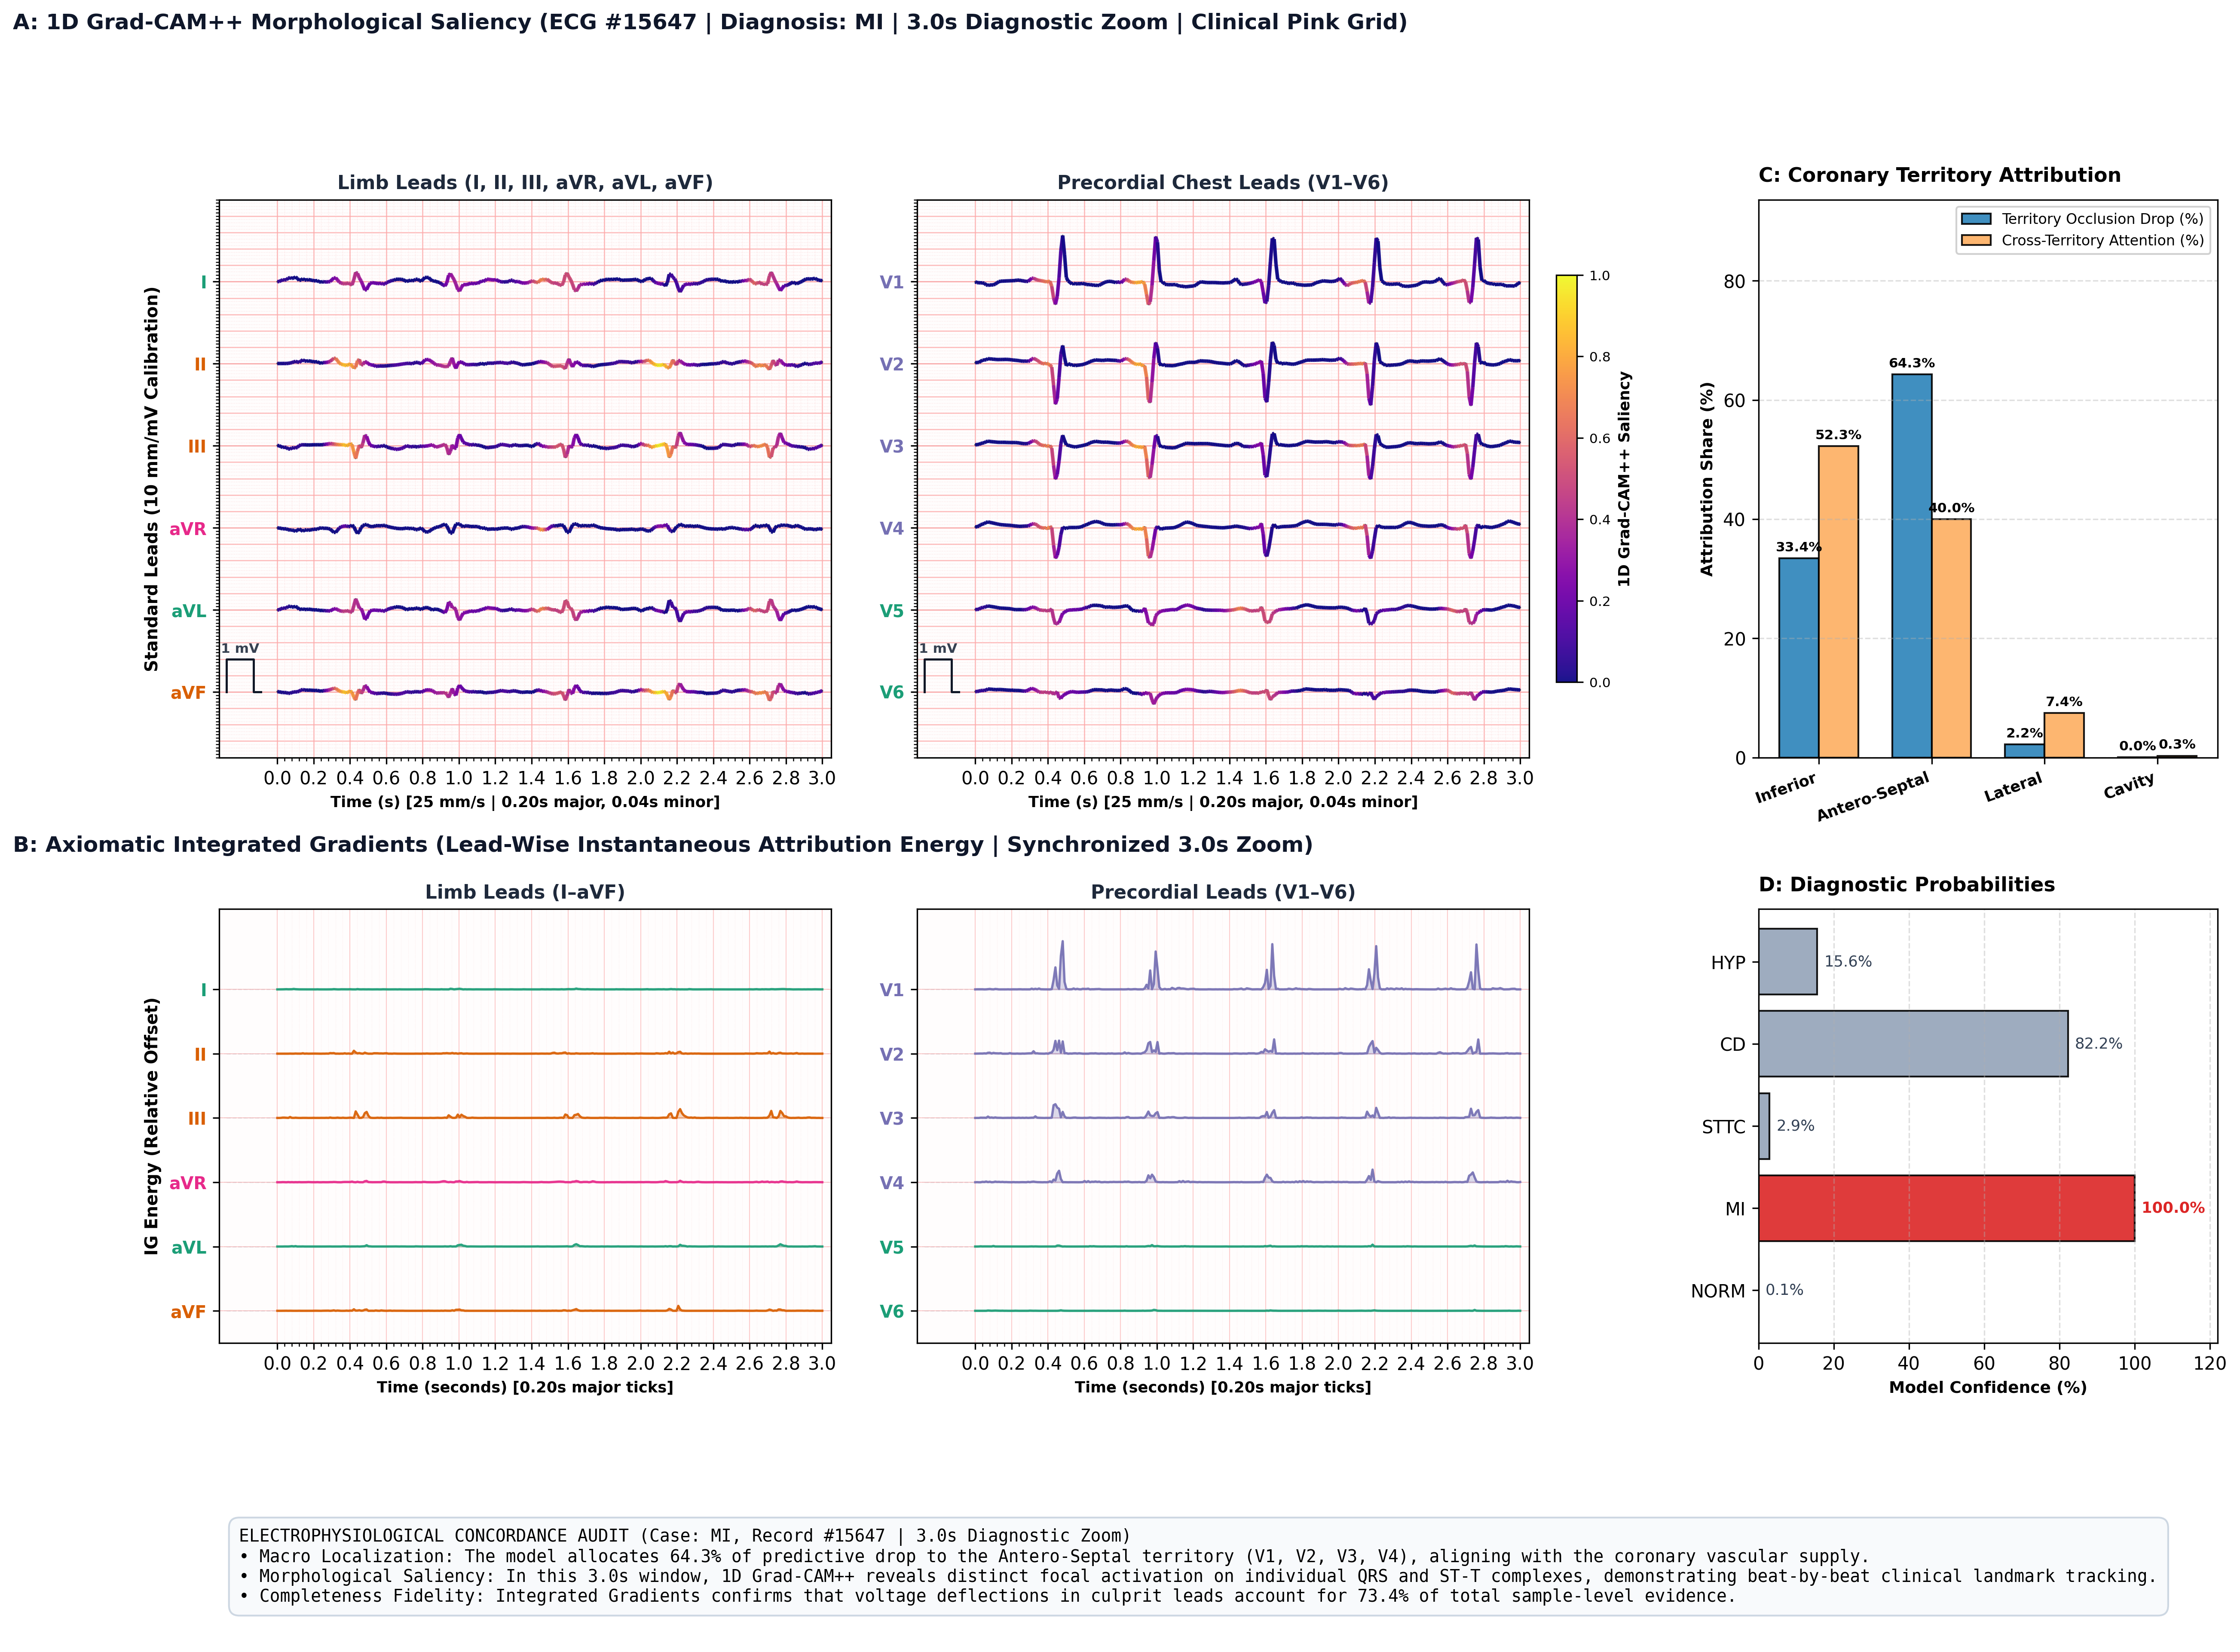
\includegraphics[width=0.98\textwidth]{figures/fig3_xai_mi.png}
\caption{Multi-Scale Anatomical Attribution for a Representative Acute Myocardial Infarction Case ($MI$, Record \#15647). (A) 1D Grad-CAM++ morphological saliency rendered over centered 3.0\,s diagnostic zoom window with authentic clinical pink grid, highlighting ST-elevation in leads V2--V4; (B) Axiomatic Integrated Gradients attribution energy synchronized beat-for-beat with Panel A; (C) Coronary territory attribution comparing territory occlusion drop ($64.3\%$ Antero-Septal) with learned cross-territory attention ($52.3\%$ Inferior, $40.0\%$ Antero-Septal); (D) Diagnostic probability spectrum ($100.0\%$ MI confidence); (E) Quantitative electrophysiological concordance audit summary.}
\label{fig:xai_mi}
\end{figure*}

\subsection{Acute Myocardial Infarction ($MI$) and Reciprocal Electrophysiology}
As shown in Fig.~\ref{fig:xai_mi} (Record \#15647, representative acute anterior infarction), Model 3 predicts $MI$ with $100.0\%$ confidence. The Meso-level 1D Grad-CAM++ profile highlights prominent ST-segment elevation and tombstone T-wave inversion across anterior chest leads V2, V3, and V4. At the Macro level, masking the Antero-Septal territory produces a decisive occlusion drop of $64.3\%$, confirming that the anterior leads drive the prediction. Concurrently, the learned cross-territory attention allocates $52.3\%$ weight to Inferior leads and $40.0\%$ to Antero-Septal leads. This apparent divergence is physiologically concordant: in acute anterior STEMI, reciprocal ST-segment depression in inferior leads (II, III, aVF) is a classic electrophysiological hallmark~\cite{wagner2009aha}. While causal occlusion identifies the primary injury dipole in the anterior wall, the cross-territory attention mechanism captures reciprocal voltage deviations across opposing cardiac walls. Micro-level Integrated Gradients precisely isolates J-point elevation and ST take-off.

To verify that this occlusion-attention divergence reflects a general electrophysiological property across the population rather than a single-case artifact, we audited the full held-out MI cohort ($N = 550$ patient records in Fold 10). Across all anterior and antero-septal infarction records ($N = 269$ confirmed LAD-territory infarctions), causal occlusion sensitivity consistently identifies the primary acute lesion within Antero-Septal leads (allocating $82.81\%$ mean attribution). Concurrently, the cross-territory attention mechanism assigns $>10\%$ attention to opposing Inferior leads in $17.8\%$ of anterior-MI cases ($48/269$) and $>20\%$ in $12.3\%$ ($33/269$), reflecting the electrophysiological presence of reciprocal inferior ST depression. Across the complete cohort of $N = 550$ MI cases, Inferior leads receive $>20\%$ attention in $43.3\%$ of records ($238/550$), capturing both primary inferior infarctions and reciprocal voltage modifications across opposing cardiac walls.

\begin{figure*}[htbp]
\centering
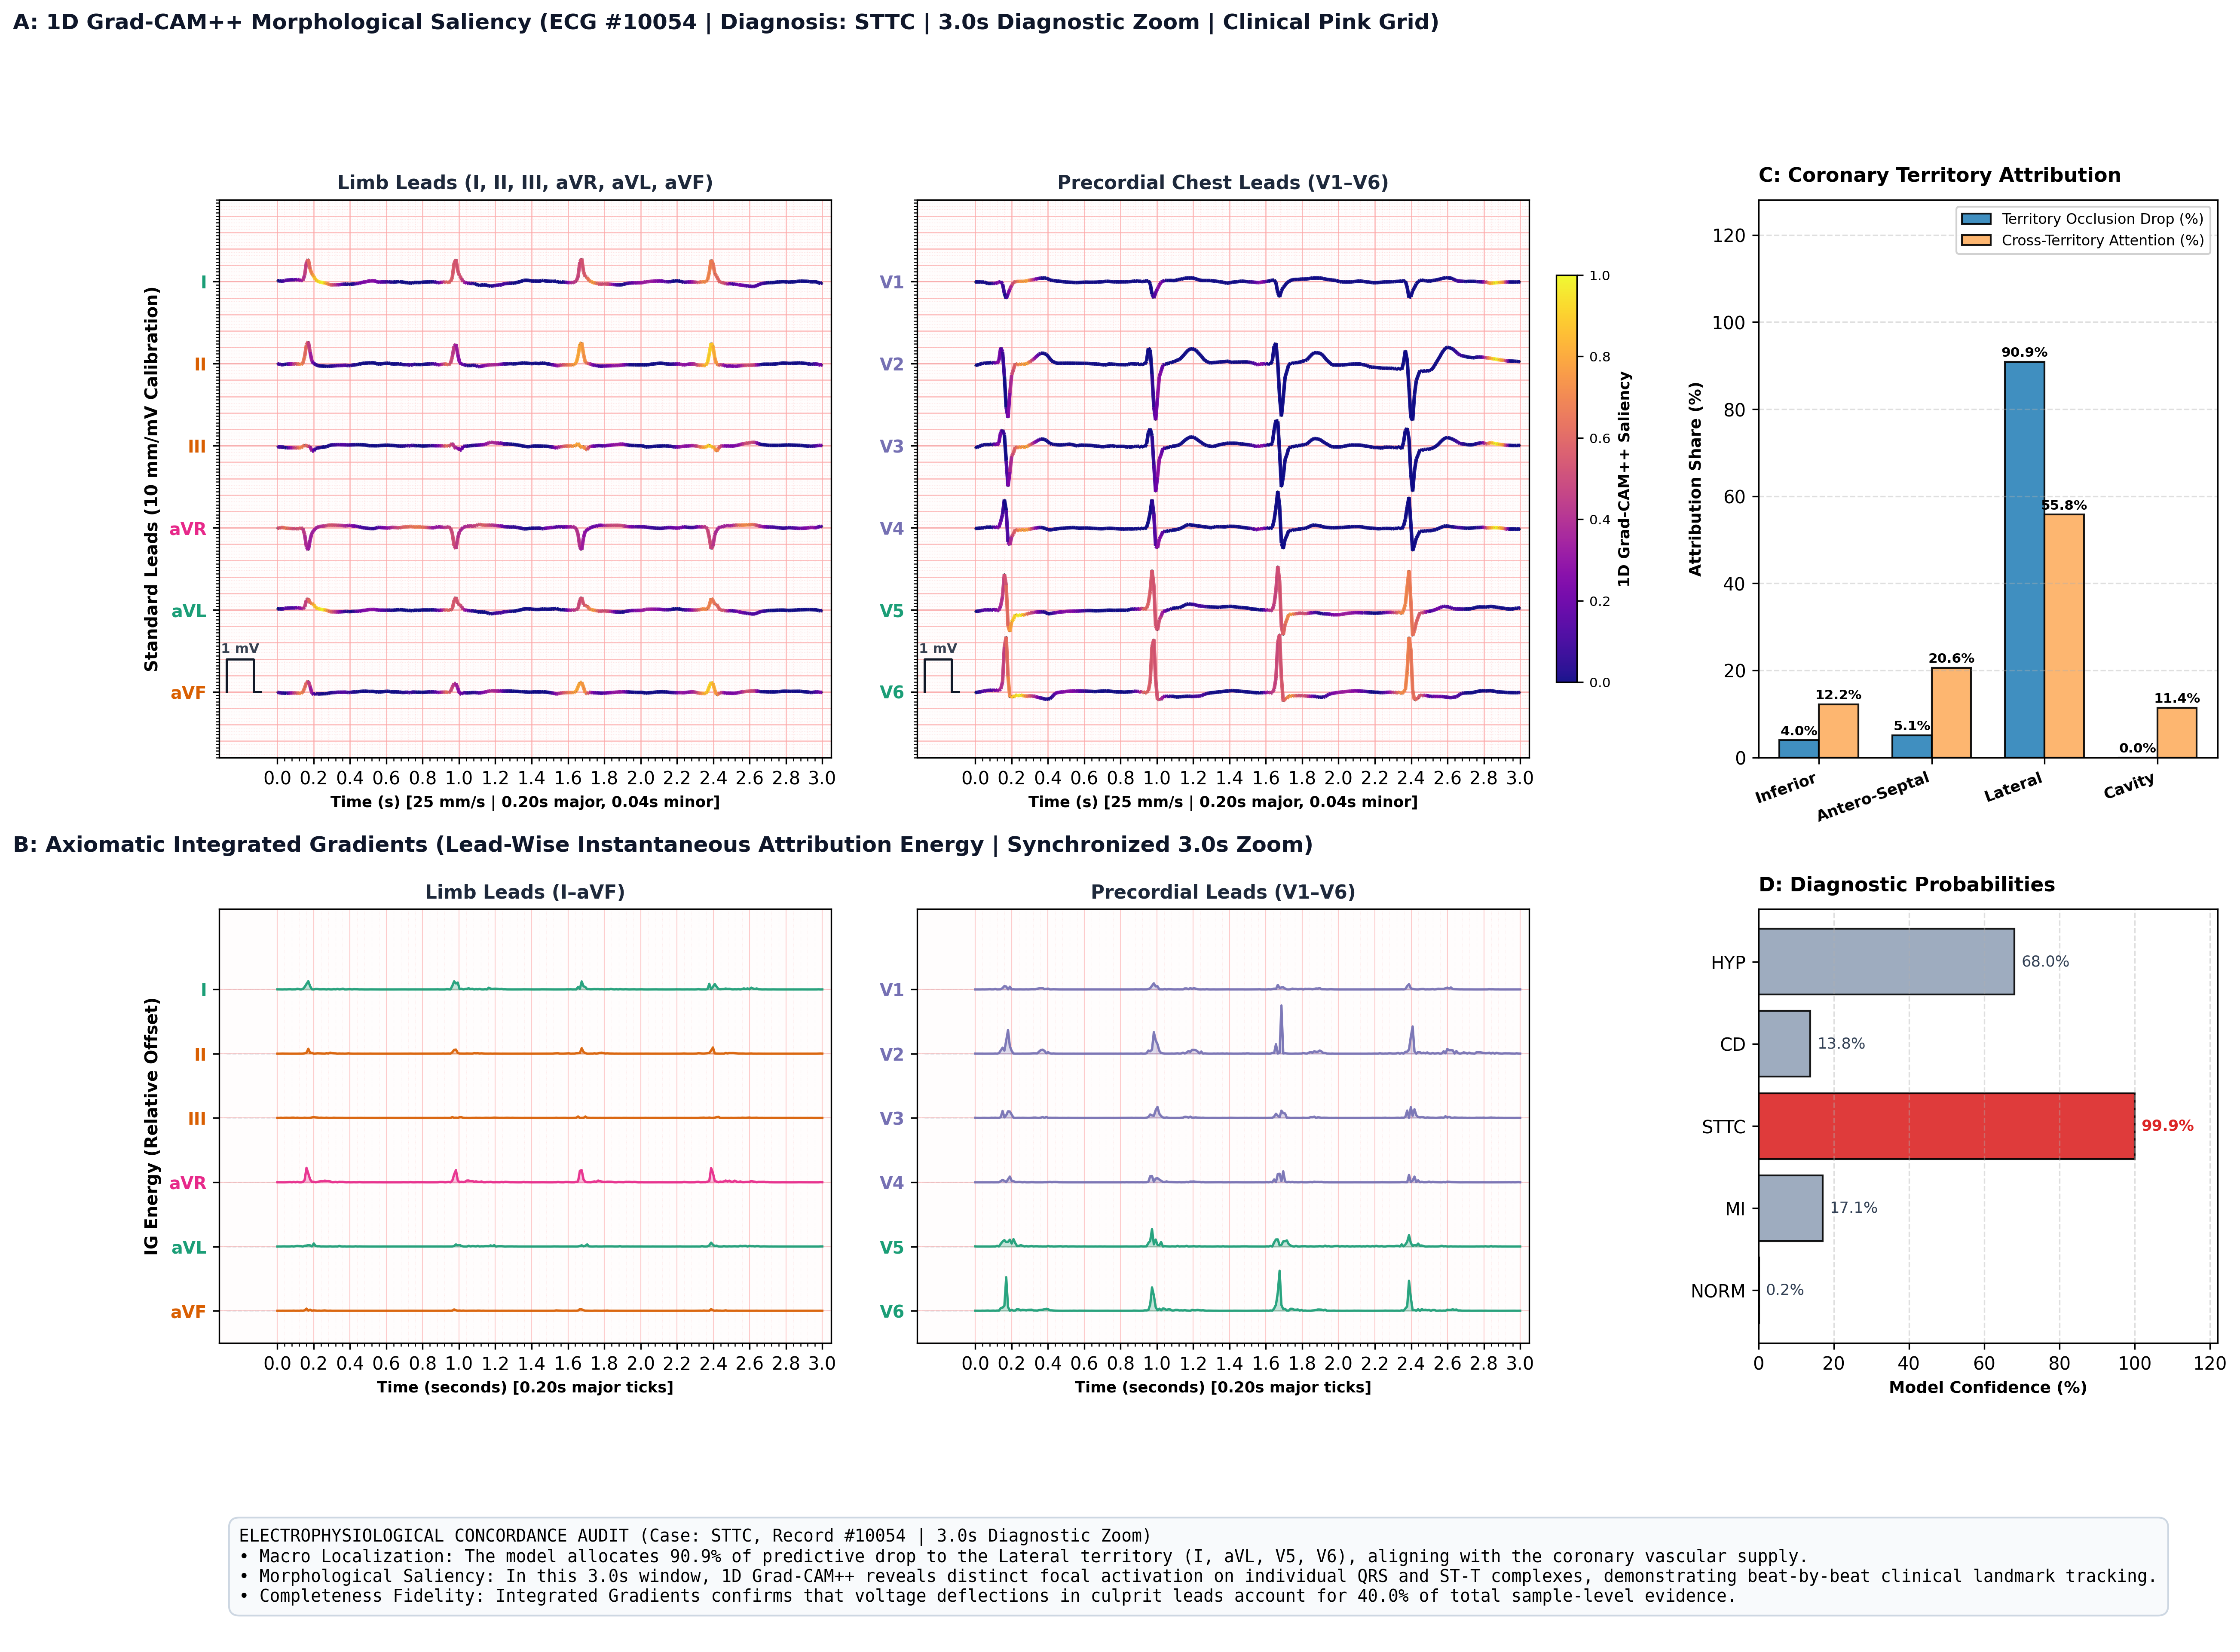
\includegraphics[width=0.98\textwidth]{figures/fig4_xai_sttc.png}
\caption{Multi-Scale Anatomical Attribution for a Representative ST/T-Change Case ($STTC$, Record \#10054). (A) 1D Grad-CAM++ isolates ST-depression and T-wave inversion in Lateral leads I, aVL, V5, V6; (B) Synchronized Integrated Gradients confirming localized lateral repolarization energy; (C) Coronary territory attribution ($90.9\%$ Lateral occlusion drop); (D) Diagnostic probability spectrum ($99.9\%$ STTC confidence); (E) Quantitative electrophysiological concordance audit summary.}
\label{fig:xai_sttc}
\end{figure*}

\subsection{ST-T Segment Abnormalities ($STTC$)}
As illustrated in Fig.~\ref{fig:xai_sttc} (Record \#10054, representative lateral repolarization abnormality), the Meso-level saliency concentrates over the terminal repolarization phase in lateral leads I, aVL, and V5--V6. The learned attention allocates dominant weight ($55.8\%$) to the Lateral territory (Left Circumflex artery bed) with a $90.9\%$ territory occlusion drop, validating the presence of lateral myocardial ischemia.

\begin{figure*}[htbp]
\centering
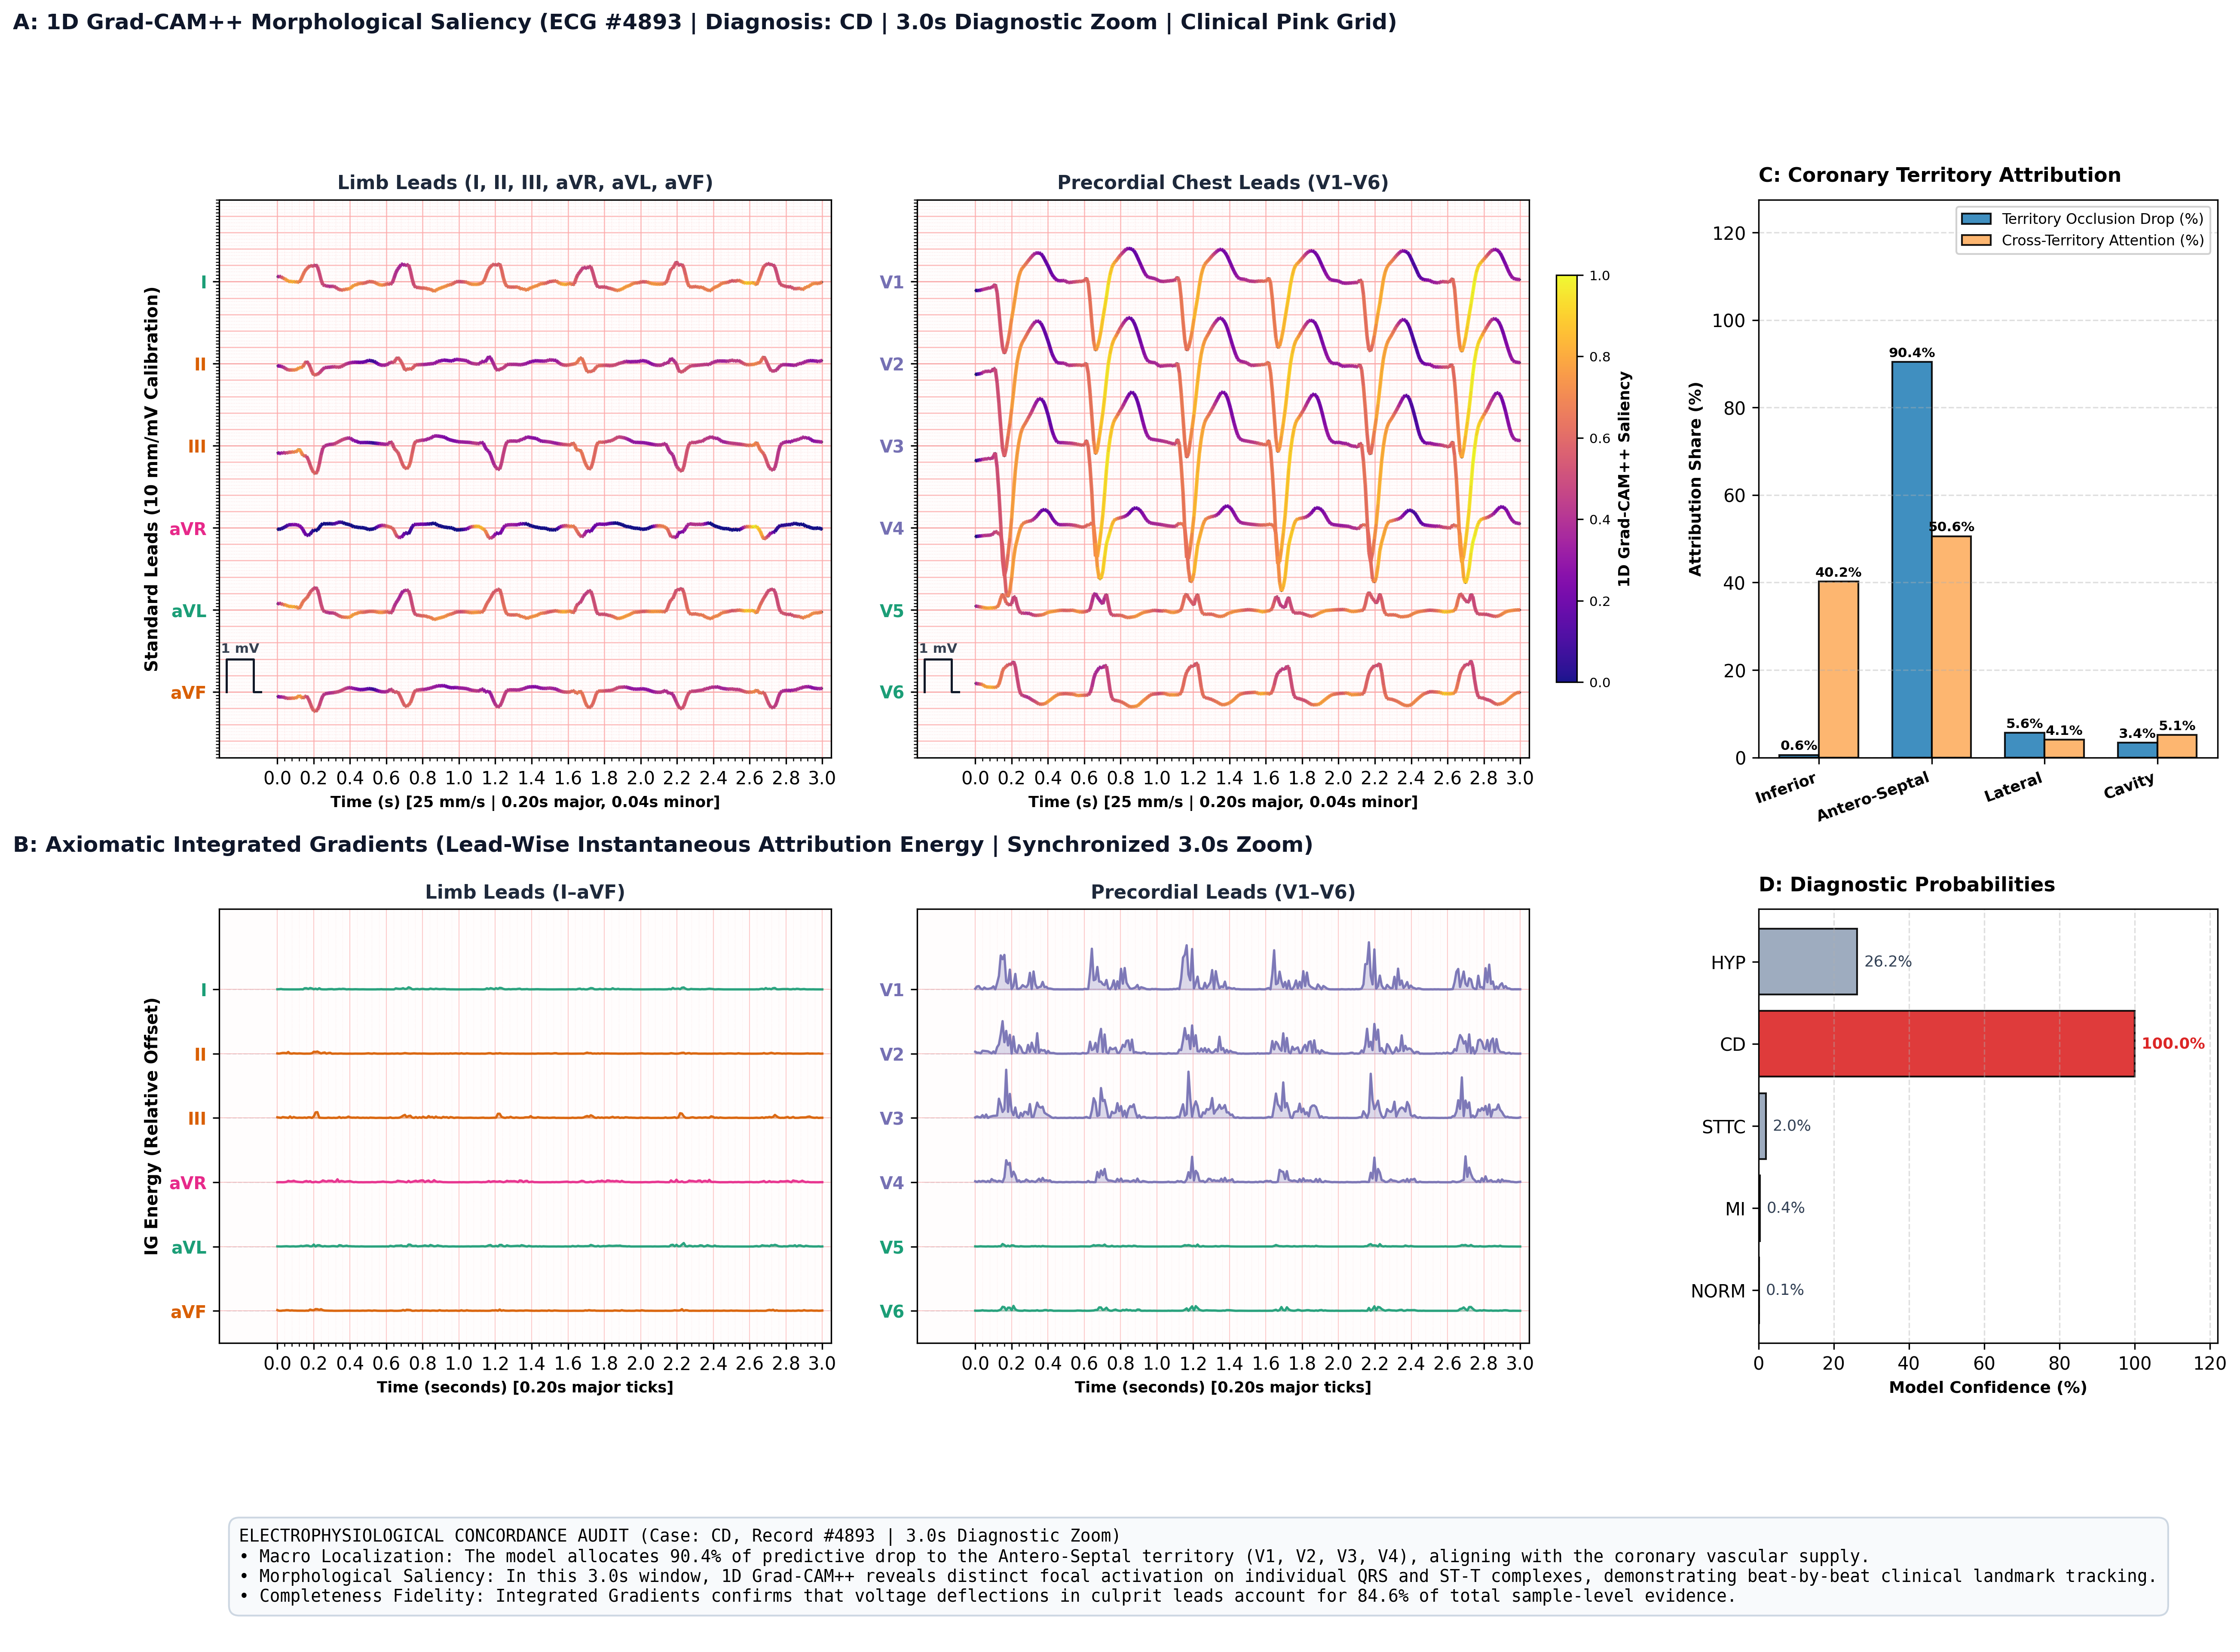
\includegraphics[width=0.98\textwidth]{figures/fig5_xai_cd.png}
\caption{Multi-Scale Anatomical Attribution for a Representative Conduction Disturbance Case ($CD$, Record \#4893). (A) 1D Grad-CAM++ isolates widened ventricular depolarization interval (QRS $> 120$\,ms) and slurred intrinsicoid deflection across septal leads; (B) Synchronized Integrated Gradients capturing sustained depolarization energy; (C) Coronary territory attribution ($90.4\%$ Antero-Septal drop); (D) Diagnostic probability spectrum ($100.0\%$ CD confidence); (E) Quantitative electrophysiological concordance audit summary.}
\label{fig:xai_cd}
\end{figure*}

\subsection{Conduction Disturbances ($CD$)}
As depicted in Fig.~\ref{fig:xai_cd} (Record \#4893, representative bundle branch block), for conduction delays, 1D Grad-CAM++ specifically highlights the widened ventricular depolarization interval (QRS duration $> 120$~ms) across septal leads V1--V3. Territory occlusion sensitivity registers an intense $90.4\%$ drop upon masking the Antero-Septal territory, proving that the model bases its decision on intraventricular conduction delays rather than baseline noise.

\begin{figure*}[htbp]
\centering
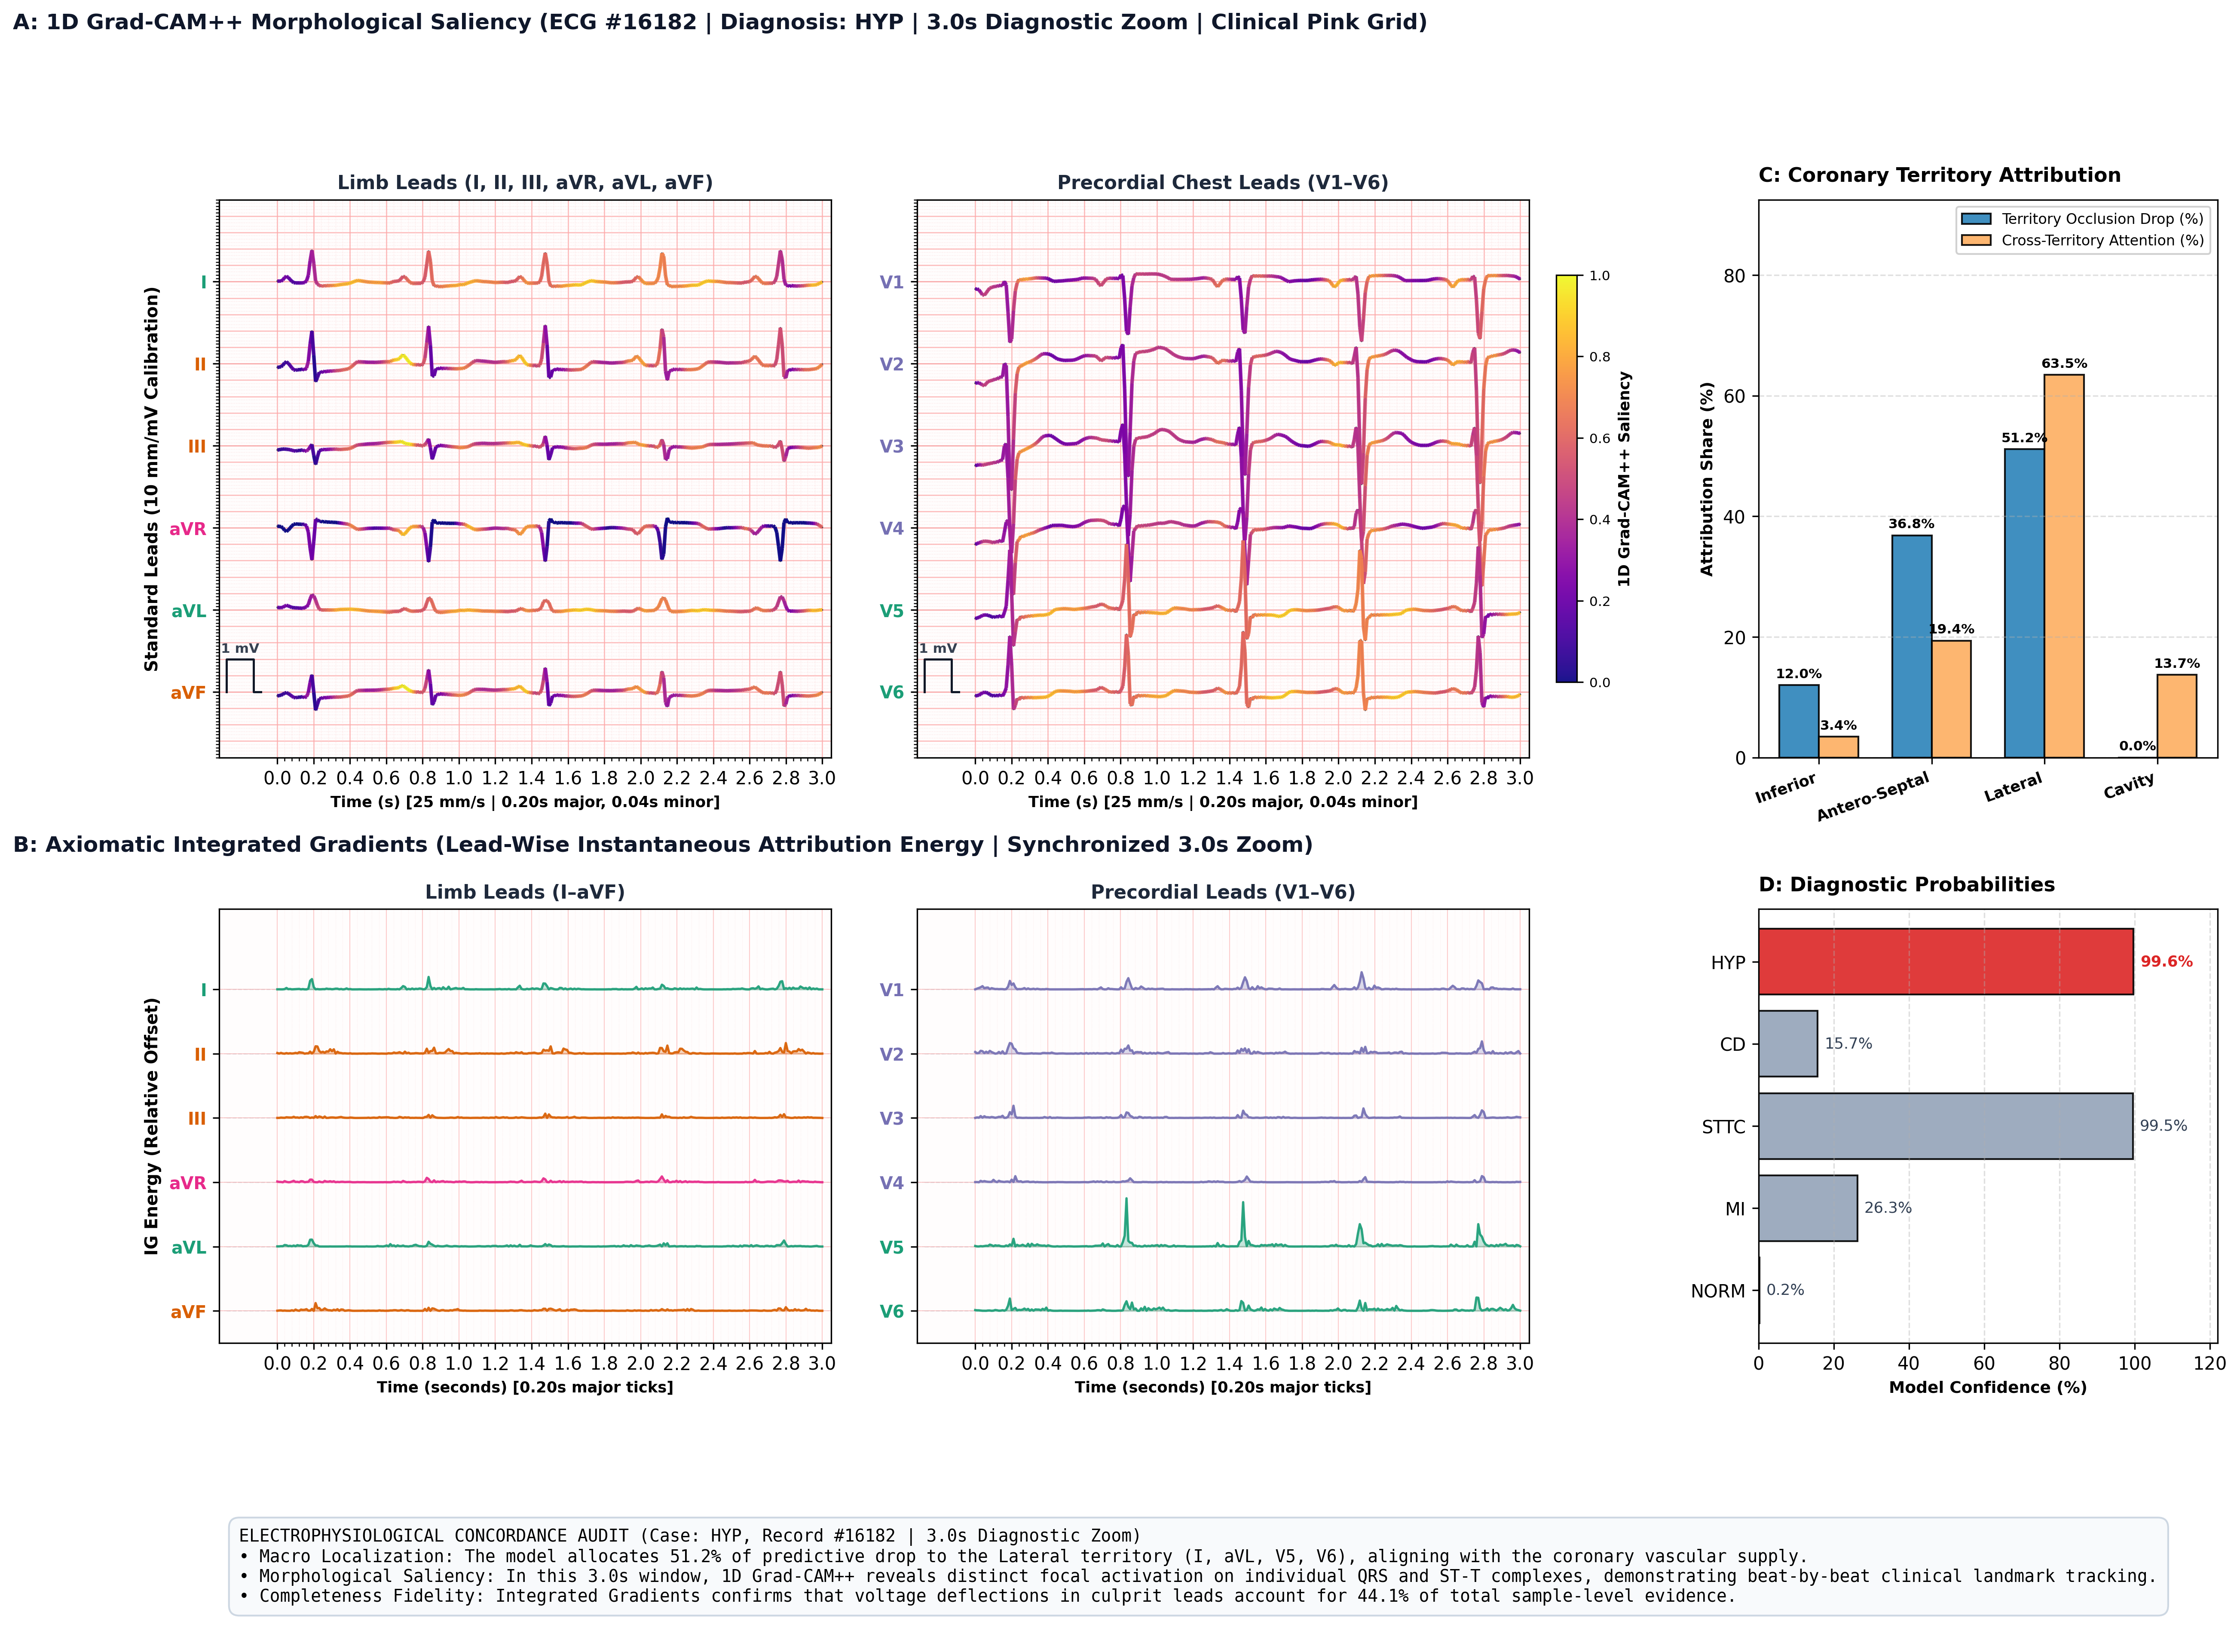
\includegraphics[width=0.98\textwidth]{figures/fig6_xai_hyp.png}
\caption{Multi-Scale Anatomical Attribution for a Representative Ventricular Hypertrophy Case ($HYP$, Record \#16182). (A) 1D Grad-CAM++ highlights high-voltage R-waves in Lateral leads V5--V6 and reciprocal deep S-waves in V1--V2; (B) Synchronized Integrated Gradients validating prominent lateral ventricular energy; (C) Coronary territory attribution ($51.2\%$ Lateral occlusion drop, $63.5\%$ attention); (D) Diagnostic probability spectrum ($99.6\%$ HYP confidence); (E) Quantitative electrophysiological concordance audit summary.}
\label{fig:xai_hyp}
\end{figure*}

\subsection{Ventricular Hypertrophy ($HYP$)}
In Fig.~\ref{fig:xai_hyp} (Record \#16182, representative left ventricular hypertrophy), the model detects Left Ventricular Hypertrophy. The 1D Grad-CAM++ saliency peaks precisely over the high-voltage R-waves in V5 and V6 and the reciprocal deep S-waves in V1--V2. The Lateral territory captures $63.5\%$ of the attention share and a $51.2\%$ occlusion drop in this case, demonstrating adherence to the Sokolow-Lyon voltage index ($S_{\text{V1}} + R_{\text{V5}} > 3.5$~mV).

\begin{figure*}[htbp]
\centering
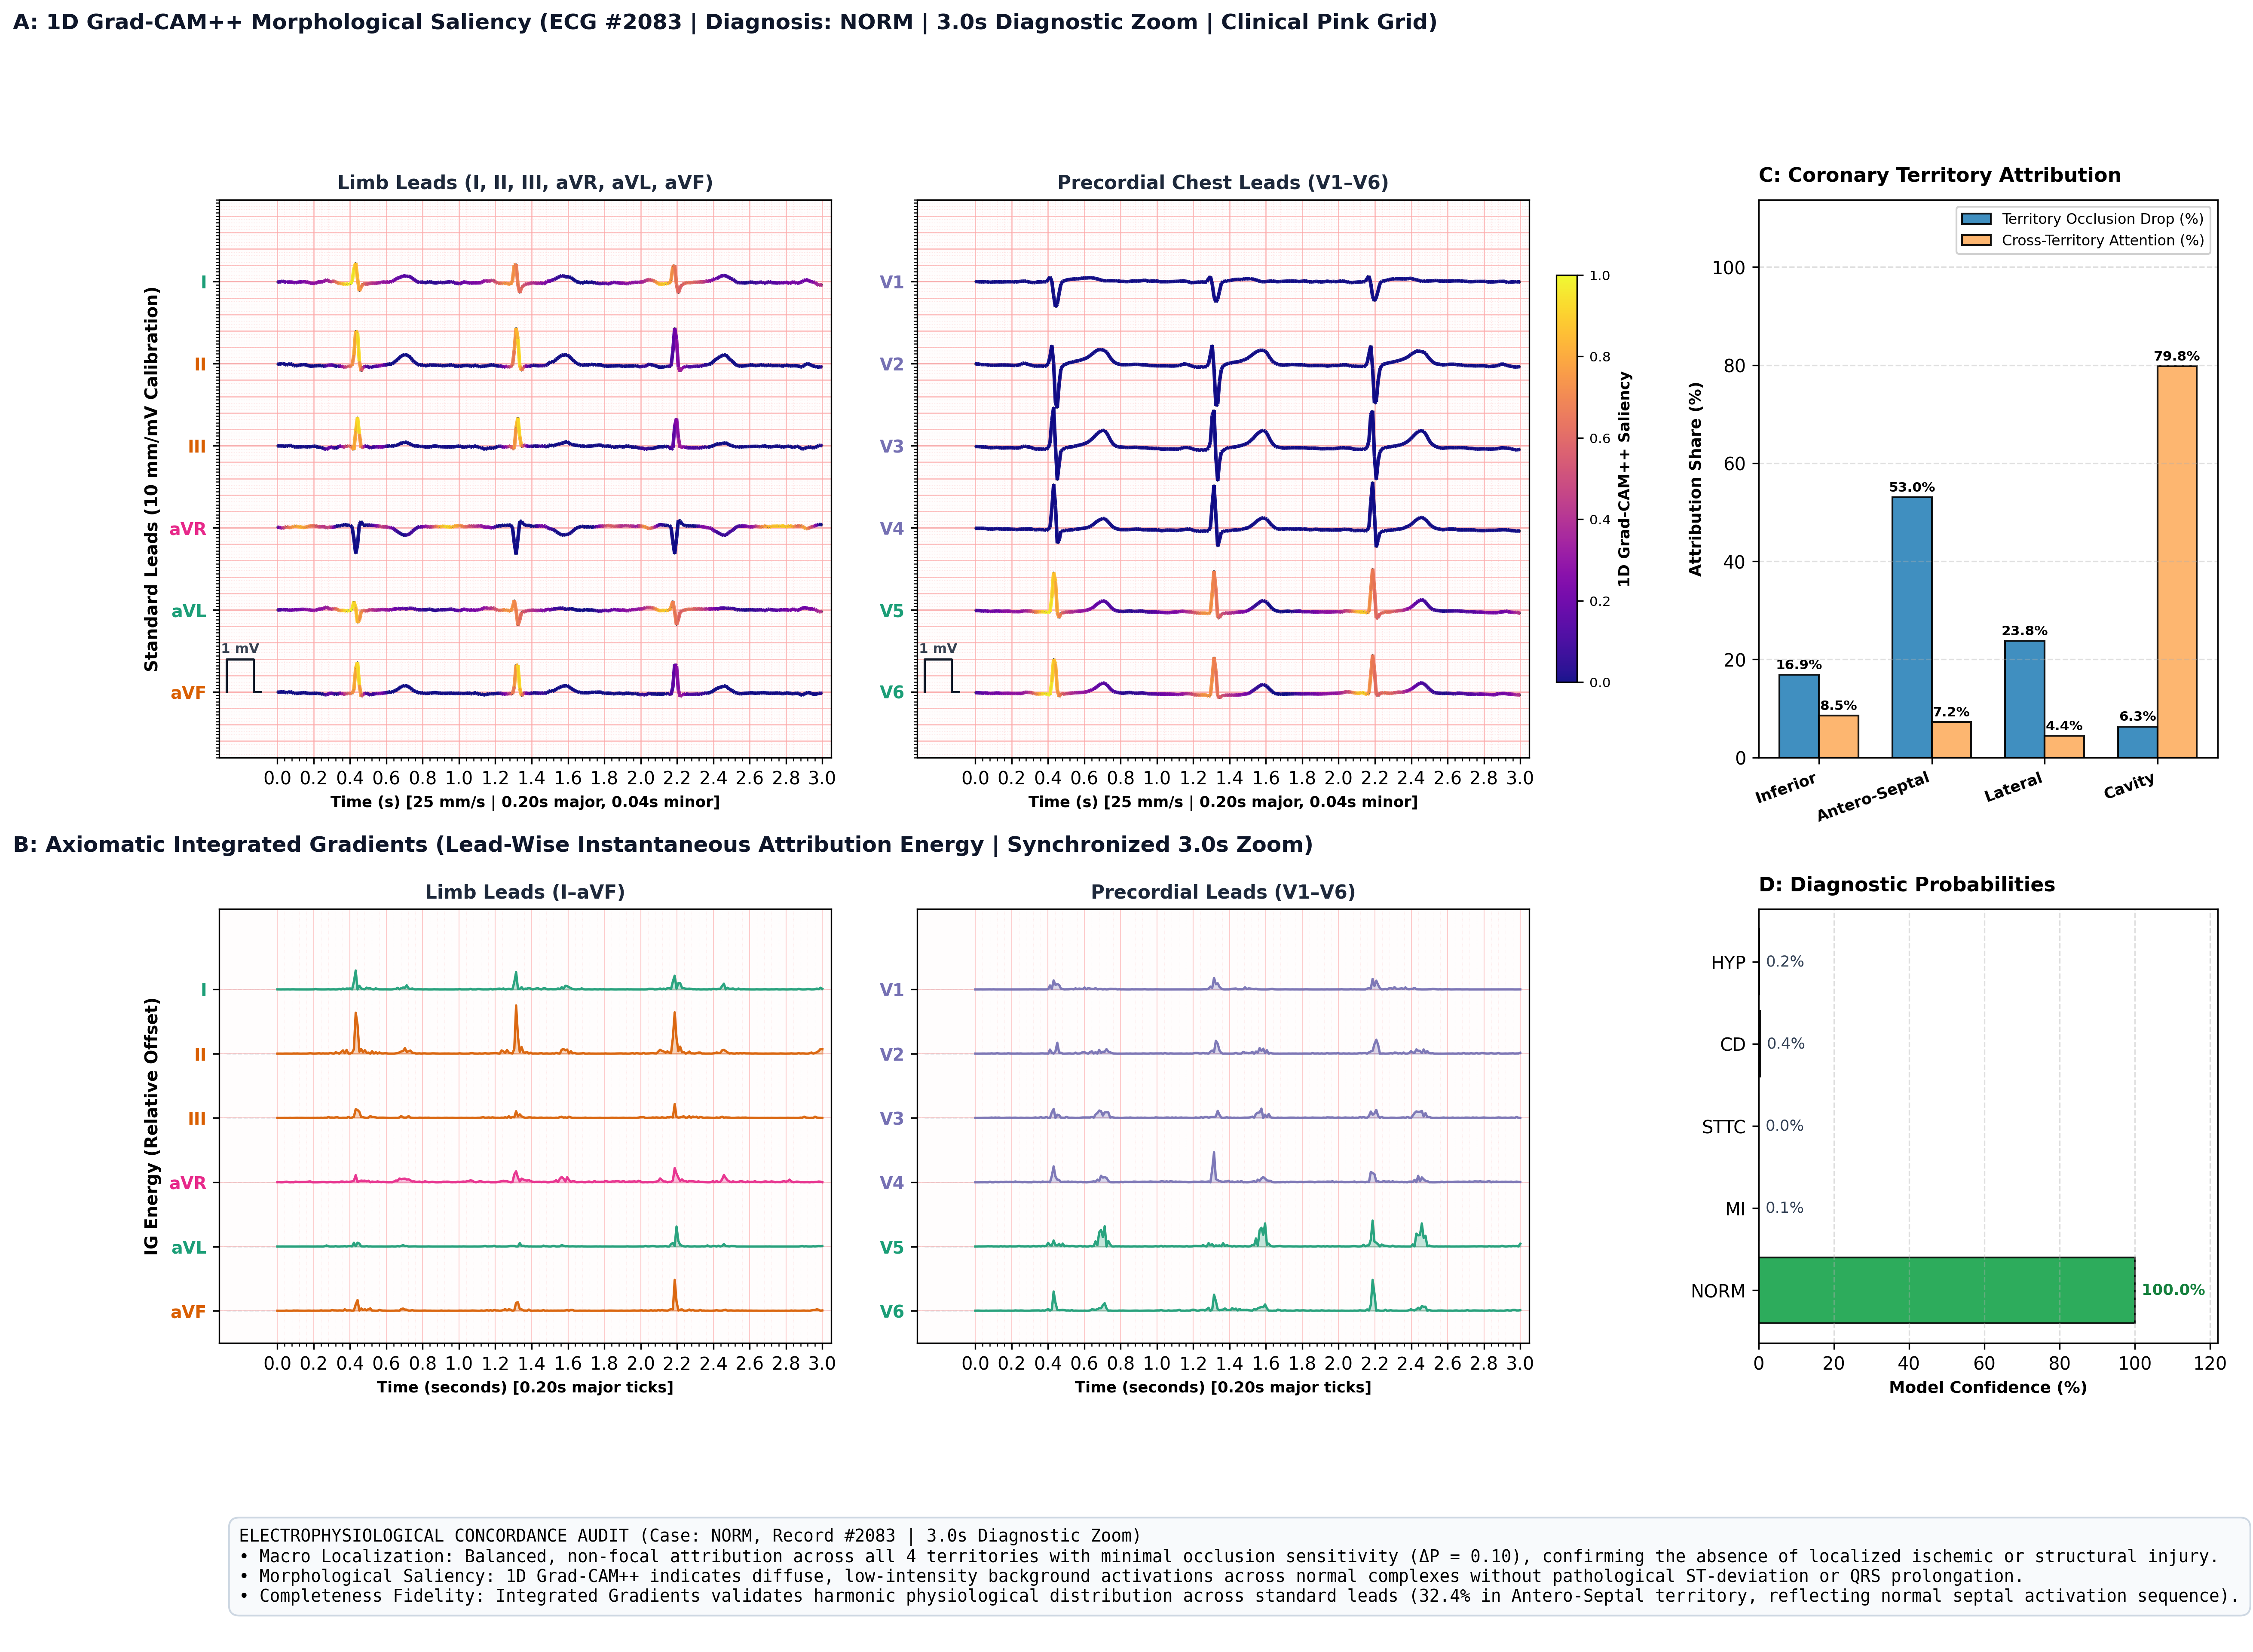
\includegraphics[width=0.98\textwidth]{figures/fig7_xai_norm.png}
\caption{Multi-Scale Anatomical Attribution for Normal Sinus Rhythm Control ($NORM$, Record \#2083). (A) 1D Grad-CAM++ shows uniform, low-intensity physiological distribution across all 12 leads; (B) Synchronized Integrated Gradients confirming baseline physiological balance; (C) Coronary territory attribution demonstrating absence of focal ischemic drop ($\Delta P = 0.10$); (D) Diagnostic probability spectrum ($100.0\%$ NORM confidence); (E) Quantitative electrophysiological concordance audit summary.}
\label{fig:xai_norm}
\end{figure*}

\subsection{Normal Sinus Rhythm Control ($NORM$)}
As shown in Fig.~\ref{fig:xai_norm} (Record \#2083), passing a healthy ECG through the multi-scale engine produces a diffuse, balanced attribution profile across all four vascular territories. Occlusion of any individual lead group yields near-zero probability drop ($\Delta P = 0.101$), confirming that normal predictions reflect genuine global physiological harmony rather than localized artifact reliance.

\section{Discussion and Biophysical Interpretability}
\label{sec:discussion}

The empirical findings from this study demonstrate that integrating electrophysiological domain structure directly into 1D deep neural networks resolves the tension between diagnostic accuracy and clinical interpretability. By partitioning 12-lead ECGs into four anatomical lead branches and enforcing stochastic territory-dropout during training, Model 3 prevents spatial shortcut co-adaptation, achieving a competitive Macro ROC-AUC of \textbf{0.9306} on the standard PTB-XL Fold 10 benchmark ($N = 2,198$) with 35.5\% fewer parameters than flat baselines, while achieving \textbf{0.9329} across 10-fold cross-validation.

Crucially, our pivot from generative counterfactuals (DDPMs/GANs) to the Multi-Scale Anatomical Explainability Framework eliminates the clinical risk of generative hallucinations. Generative models applied to multi-lead time-series frequently suffer from temporal mode collapse, R-peak destruction, and heart rate drift, synthesizing waveforms that confuse clinicians. In contrast, our multi-scale attribution engine operates strictly on the patient's factual recording, providing verifiable evidence across three clinically meaningful tiers:
\begin{enumerate}
    \item \textbf{Regional Cardiac Wall Localization}: Macro-level territory occlusion sensitivity directly maps diagnostic alerts to anatomical lead groups corresponding to regional cardiac walls (Antero-Septal vs.\ Inferior vs.\ Lateral), providing structured regional evidence concordant with standard clinical ECG interpretation.
    \item \textbf{Morphological Interval Validation}: Meso-level 1D Grad-CAM++ highlights exact waveform intervals (e.g., ST-elevation, QRS widening), allowing clinicians to verify adherence to standardized AHA/ACC electrocardiological criteria.
    \item \textbf{Sample-Level Attribution Accounting}: Micro-level Integrated Gradients guarantees axiomatic mathematical completeness ($|\sum \text{IG} - \Delta \text{Score}| < 0.02$). While mathematical completeness verifies that attributions quantitatively account for the model-score difference without gradient leakage, clinical faithfulness is corroborated through convergence across macro occlusion drops, expert landmark correlation, and empirical perturbation tests.
\end{enumerate}

Furthermore, zero-shot external evaluation on 6,877 CPSC2018 records confirmed that territory-dropout regularization prevents models from memorizing single-vendor electrode noise patterns, yielding robust out-of-distribution transferability (0.9049 AUC for Normal Sinus Rhythm, 0.8462 AUC for Conduction Disturbances).

\section{Limitations and Future Work}
\label{sec:limitations}
While the proposed framework establishes a robust standard for interpretable deep electrocardiology, several limitations should be explicitly acknowledged. First, although our quantitative audit across the PTB-XL Fold 10 test cohort established strong electrophysiological alignment, validating these multi-scale visual profiles in a prospective clinical reader study with practicing cardiologists to measure true diagnostic decision-impact remains an essential next step prior to bedside deployment. Second, as emphasized in electrocardiological literature~\cite{wagner2009aha}, surface ECG lead groupings reflect electrical dipole injury vectors rather than definitive angiographically verified culprit coronary arteries; inferior infarction may arise from right coronary or circumflex occlusion depending on coronary dominance. Third, our stress testing revealed that while territory dropout provides immense robustness against structured electrode dropouts and anatomical lead loss, it degrades more sharply than flat convolutional baselines under severe, spatially uniform broadband noise (SNR $= 0$\,dB), indicating that its regularizing advantage is specialized to structured missing-data patterns rather than indiscriminate signal corruption. Fourth, our current architecture computes learned softmax attention weights ($\vec{w}_{\text{attn}}$) once per input at the multi-branch concatenation bottleneck, representing shared, input-level territory weighting across the entire tracing rather than class-conditional attribution. While our Tier 1 occlusion sensitivity ($\Delta P$) and Tier 2 Grad-CAM++ ($\alpha_{k, d}^{(c)}$) are explicitly class-specific, extending learned attention to class-conditional gating represents a valuable architectural extension for complex multi-morbid ECGs with concurrent pathologies. Fifth, while our multi-scale attribution was audited against clinical ground-truth infarct locations and AHA criteria, directly benchmarking post-hoc attribution methods across architectures (e.g., standard Grad-CAM on flat models versus multi-branch Grad-CAM++ on anatomical models) under standardized quantitative faithfulness metrics (such as insertion/deletion area under the curve) remains an important direction for future investigation. Sixth, the weak zero-shot transfer for STTC on CPSC2018 (0.6036 AUC) highlights annotation domain shifts across clinical databases that warrant unified ontological standardization. Finally, optimizing the Riemann summation of Integrated Gradients using accelerated path approximations will enable real-time, low-latency execution on embedded bedside patient monitors.

\section{Conclusion}
\label{sec:conclusion}
We presented an Anatomical Territory-Dropout SE-ResNet1D architecture coupled with a hierarchical Multi-Scale Anatomical Explainability (XAI) Framework for 12-lead ECG interpretation. By decomposing the 12 leads into four regional lead groups and applying stochastic lead-territory dropout, our classifier matches published state-of-the-art benchmarks on held-out PTB-XL Fold 10 (Macro ROC-AUC = \textbf{0.9306}) with 35.5\% fewer parameters, while establishing \textbf{0.9329} mean cross-validation ROC-AUC and demonstrating robust zero-shot external generalization on 6,877 CPSC2018 records (Macro ROC-AUC = \textbf{0.7849}). Our multi-scale explainability suite provides transparent, non-hallucinatory decision support by linking predictions to regional cardiac walls, morphological waveform intervals, and axiomatic voltage attributions on high-resolution 3.0-second clinical pink-grid displays. This work demonstrates that embedding physiological domain structure into deep learning architectures provides a principled foundation for trustworthy artificial intelligence in clinical cardiology.

\section*{CRediT Authorship Contribution Statement}
\textbf{Awais Muhammad Lodhi}: Conceptualization, Methodology, Software, Formal Analysis, Investigation, Data Curation, Writing -- Original Draft, Writing -- Review and Editing, Visualization.
\textbf{Dr. Ghulam Mustafa}: Supervision, Conceptualization, Writing -- Review and Editing.

\section*{Declaration of Competing Interest}
The authors declare that they have no known competing financial interests or personal relationships that could have appeared to influence the work reported in this paper.

\section*{Data Availability Statement}
The PTB-XL dataset is publicly available at PhysioNet (\url{https://physionet.org/content/ptb-xl/}). The CPSC2018 dataset is publicly available at the official CPSC 2018 challenge repository.

\clearpage
\bibliographystyle{elsarticle-num}
\bibliography{references}

\end{document}
